\documentclass[12pt]{article}

\usepackage {fullpage}
%\usepackage {palatino}
\usepackage {epsfig}
\usepackage{amsmath}
\usepackage{amssymb}
\usepackage{amsfonts}
\usepackage{url}
\textwidth 6.5in
\topmargin 0in \headheight 0in
%\headsep 0.5in
\textheight 8.7in
\oddsidemargin 0in
\evensidemargin 0in
\parskip 0.1in
\parindent 0in

\pagestyle{empty}

\def\beqa#1\eeqa{\begin{eqnarray}#1\end{eqnarray}}
\newcommand{\bmu}{{\boldsymbol{\mu}}}
\newcommand{\bSigma}{{\boldsymbol{\Sigma}}}
\newcommand{\bx}{{\bf{x}}}


\newcommand{\items}{\vspace{-.25in}\begin{itemize}\setlength{\itemsep}{1mm}}
\newcommand{\degree}{{\raisebox{.6ex}[0ex][0ex]{\small $\circ$}}}
\newcommand{\cut}[1]{}
\newcommand{\eg}{{\it eg \/}}
\newcommand{\ie}{{\it ie \/}}
\newcommand{\bighead}[1]{\begin{slide}\begin{center}{\bf \large
\underline{#1}}\end{center}}
\newcommand{\numbs}{\vspace{-.25in}\begin{enumerate}\setlength{\itemsep}{1mm}}
\newcommand{\itemss}{\vspace{-.05in}\begin{itemize}\setlength{\itemsep}{1mm}}

\newcommand{\indentit}{\mbox{  }\hspace{.1in}}
\newcommand{\vbon}{\begin{verbatim}}
\newcommand{\vboff}{\end{verbatim}}
\renewcommand{\vec}[1]{\boldsymbol{#1}}
\newcommand{\yy}{\mathbf{y}}
\newcommand{\xx}{\mathbf{x}}
\newcommand{\zz}{\mathbf{z}}
\newcommand{\ttt}{\mathbf{t}}
\newcommand{\dd}[2]{\frac{\partial #1}{\partial #2}}
\newcommand{\pderi}[2]{\frac{\partial #1}{\partial #2}}
\newcommand{\deri}[2]{\frac{{\rm d} #1}{{\rm d} #2}}
\DeclareMathOperator{\E}{\mathbb{E}}
\DeclareMathOperator{\cov}{cov}
\DeclareMathOperator{\diag}{diag}

\begin{document}

\begin{center}
{\bf CSC 411}\\
{\bf Introduction to Machine Learning}\\
{\large \bf Assignment 2}\\
{\bf Farzad Niroui}\\
{\bf *********}
\end{center}

\section{EM for Mixture of Gaussians}

Given that the Gaussian mixture model is:
\beqa
 p(\bx) = \sum_{k=1}^K \pi_k {\cal{N}}(\bx | \bmu_k, \bSigma_k)
\eeqa

Additional, given the special case in which the covariance matrix $\bSigma_k = \bSigma$, for all $k$, we can derive the EM equations for maximizing the likelihood function. 

\subsection*{E step:}
The conditional probability of $z$ given $x$ (responsibility) is as follows:

\begin{equation}\label{res}
\begin{split}
\gamma_k = p(z=k|x) & = \frac{p(z=k)p(x|z=k)}{p(x)} \\
&= \frac{p(z=k)p(x|z=k)}{\sum_{j=1}^K \pi_j {\cal{N}}(\bx | \bmu_j, \bSigma_j)} \\
&= \frac{\pi_k {\cal{N}}(\bx | \bmu_k, \bSigma_k)}{\sum_{j=1}^K \pi_j {\cal{N}}(\bx | \bmu_j, \bSigma_j)} \\
\end{split}
\end{equation}

\subsection*{M step:}
Taking the log-likelihood of the GMM:

\begin{equation}\label{like}
ln p(X|\pi,\bmu,\bSigma) = \sum_{n=1}^N ln \sum_{k=1}^K \pi_k {\cal{N}}(\bx^{(n)}| \bmu_k, \bSigma_k)
\end{equation}

Given the Gaussian model ${\cal{N}}(\bx | \bmu, \bSigma) = \frac{1}{\sqrt{(2\pi)^d|\bSigma|}}exp(-\frac{1}{2}(x-\bmu)^T\bSigma^{-1}(x-\bmu))$ and the property of $\frac{\partial x^TAx}{\partial x} = x^T(A+A^T)$, we can set the derivative of Equation \ref{like} to 0 and compute the partial derivative with respect to $\bmu_k$. We also know that $\bSigma = \bSigma^T$, therefore $\bSigma^{-1} = (\bSigma^{-1})^T$ due to the covariance matrix being symmetrical. 

\begin{equation}\label{dermu}
\begin{split}
\frac{\partial ln p(X|\pi,\bmu,\bSigma)}{\partial \bmu_k} = 0 &= \sum_{n=1}^N 
\frac{\pi_k}{\sum_{j=1}^K \pi_j {\cal{N}}(\bx | \bmu_j, \bSigma_j)}
\frac{\partial {\cal{N}}(\bx^{(n)} | \bmu_k, \bSigma_k)}{\partial \bmu_k} \\
&=\sum_{n=1}^N \frac{\pi_k {\cal{N}}(\bx^{(n)} | \bmu_k, \bSigma_k)}{\sum_{j=1}^K \pi_j {\cal{N}}(\bx | \bmu_j, \bSigma_j)} \frac{\partial (-\frac{1}{2}(x^{(n)}-\bmu_k)^T\bSigma^{-1}(x^{(n)}-\bmu_k))}{\partial \bmu_k} \\
&=\sum_{n=1}^N \frac{\pi_k {\cal{N}}(\bx^{(n)} | \bmu_k, \bSigma_k)}{\sum_{j=1}^K \pi_j {\cal{N}}(\bx | \bmu_j, \bSigma_j)} \frac{(x^{(n)}-\bmu_k)^T(\bSigma^{-1}+(\bSigma^{-1})^T)}{2} \\
&=\sum_{n=1}^N \frac{\pi_k {\cal{N}}(\bx^{(n)} | \bmu_k, \bSigma_k)}{\sum_{j=1}^K \pi_j {\cal{N}}(\bx | \bmu_j, \bSigma_j)} (x^{(n)}-\bmu_k)^T\bSigma^{-1} \\
&=\sum_{n=1}^N \frac{\pi_k {\cal{N}}(\bx^{(n)} | \bmu_k, \bSigma_k)}{\sum_{j=1}^K \pi_j {\cal{N}}(\bx | \bmu_j, \bSigma_j)} \bSigma^{-1}(x^{(n)}-\bmu_k) \\
&=\sum_{n=1}^N \gamma_k^{(n)} \bSigma^{-1}(x^{(n)}-\bmu_k) \\
\end{split}
\end{equation}

Now we can solve for the closed form updates for $\bmu_k$. Once again we note that $\bSigma_k = \bSigma$, for all $k$.

\begin{equation}\label{dermu}
\begin{split}
\sum_{n=1}^N \gamma_k^{(n)} \bSigma^{-1}(\bmu_k) = \sum_{n=1}^N \gamma_k^{(n)} \bSigma^{-1}(x^{(n)}) \\ 
N_k\bmu_k = \sum_{n=1}^N \gamma_k^{(n)}x^{(n)} \\
\bmu_k = \frac{1}{N_k}\sum_{n=1}^N \gamma_k^{(n)}x^{(n)} \\ 
\end{split}
\end{equation}

Where $N_k=\sum_{n=1}^N \gamma_k^{(n)}$.

Similarly, we can derive the we can set the partial derivative of Equation \ref{like} to 0 and compute the partial derivative with respect to $\bSigma$. The helpful properties for this derivation are $\frac{d|x|}{dx}=|x|(x^{-1})^T$ and $\frac{dx^{-1}}{dx}=-x^{-1}x^{-1}$

\begin{equation}\label{derSig}
\begin{split}
\frac{\partial {\cal{N}}(\bx^{(n)} | \bmu_k, \bSigma_k)}{\partial \bSigma}&=\frac{-1}{2}\frac{exp(...)(-\bSigma^{-1}(x^{(n)}-\bmu_k)(x^{(n)}-\bmu_k)^T\bSigma^{-1}))}{\sqrt{(2\pi)^d|\bSigma|}} + \frac{-1}{2}\frac{exp(...)(2\pi)^d|\bSigma|\bSigma^{-1}}{(2\pi)^d|\bSigma|} \\
&=\frac{-1}{2}{\cal{N}}(\bx^{(n)} | \bmu_k, \bSigma_k)[(-\bSigma^{-1}(x^{(n)}-\bmu_k)(x^{(n)}-\bmu_k)^T\bSigma^{-1})^T + \bSigma^{-1}]
\end{split}
\end{equation}

\begin{equation}\label{derSig}
\begin{split}
\frac{\partial ln p(X|\pi,\bmu,\bSigma)}{\partial \bSigma} = 0 
&= \sum_{n=1}^N\frac{\pi_k}{\sum_{j=1}^K \pi_j {\cal{N}}(\bx | \bmu_j, \bSigma_j)}
\frac{\partial {\cal{N}}(\bx^{(n)} | \bmu_k, \bSigma_k)}{\partial \bSigma} \\
&=\frac{-1}{2}\sum_{n=1}^N \frac{\pi_k {\cal{N}}(\bx^{(n)} | \bmu_k, \bSigma_k)}{\sum_{j=1}^K \pi_j {\cal{N}}(\bx | \bmu_j, \bSigma_j)}[(-\bSigma^{-1}(x^{(n)}-\bmu_k)(x^{(n)}-\bmu_k)^T\bSigma^{-1})^T + \bSigma^{-1}] \\
&=\frac{-1}{2}\sum_{n=1}^N\gamma_k^{(n)}[(-\bSigma^{-1}(x^{(n)}-\bmu_k)(x^{(n)}-\bmu_k)^T\bSigma^{-1})^T + \bSigma^{-1}] \\
&=\sum_{n=1}^N\gamma_k^{(n)}\bSigma^{-1}[(-\bSigma^{-1}(x^{(n)}-\bmu_k)(x^{(n)}-\bmu_k)^T)^T + 1] \\
\end{split}
\end{equation}

\begin{equation}\label{derSig}
\begin{split}
\sum_{n=1}^N\gamma_k^{(n)}&=\sum_{n=1}^N\gamma_k^{(n)}[(\bSigma^{-1}(x^{(n)}-\bmu_k)(x^{(n)}-\bmu_k)^T)^T] \\
\sum_{n=1}^N\gamma_k^{(n)}&=\sum_{n=1}^N\gamma_k^{(n)}[(x^{(n)}-\bmu_k)(x^{(n)}-\bmu_k)^T\bSigma^{-1}] \\
\sum_{n=1}^N\gamma_k^{(n)}\bSigma&=\sum_{n=1}^N\gamma_k^{(n)}(x^{(n)}-\bmu_k)(x^{(n)}-\bmu_k)^T \\
\bSigma&=\frac{1}{N_k}\sum_{n=1}^N\gamma_k^{(n)}(x^{(n)}-\bmu_k)(x^{(n)}-\bmu_k)^T 
\end{split}
\end{equation}

Where $N_k=\sum_{n=1}^N \gamma_k^{(n)}$.

To derive the equation for the mixing coefficient $\pi_k$ we repeat the same procedure as before but now we must consider the identity that $\sum_{k=1}^K\pi_k=1$ and use a Lagrange multiplier and maximize the following expression:
\begin{equation}\label{derSig}
\begin{split}
&lnp(X|\pi,\bmu,\bSigma)+\lambda(\sum_{k=1}^K\pi_k-1)\\
0&=\sum_{n=1}^N \frac{{\cal{N}}(\bx^{(n)} | \bmu_k, \bSigma_k)}{\sum_{j=1}^K \pi_j {\cal{N}}(\bx | \bmu_j, \bSigma_j)} +\lambda \\
\lambda&=-\sum_{n=1}^N \frac{{\cal{N}}(\bx^{(n)} | \bmu_k, \bSigma_k)}{\sum_{j=1}^K \pi_j {\cal{N}}(\bx | \bmu_j, \bSigma_j)} \\
\pi_k\lambda&=-\sum_{n=1}^N \frac{\pi_k{\cal{N}}(\bx^{(n)} | \bmu_k, \bSigma_k)}{\sum_{j=1}^K \pi_j {\cal{N}}(\bx | \bmu_j, \bSigma_j)} \\
\sum_{k=1}^K\pi_k\lambda&=-\sum_{k=1}^K\sum_{n=1}^N \gamma_k^{(n)} \\
\lambda &= -N \\
\pi_k\lambda&=-N_k \\
\pi_k(-N)&=-N_k \\
\pi_k&=\frac{N_k}{N} \\
\end{split}
\end{equation}

Where $N_k=\sum_{n=1}^N \gamma_k^{(n)}$. 

\newpage
\section{Convolutional Neural Networks}
\begin{figure}[!htb]
\centering
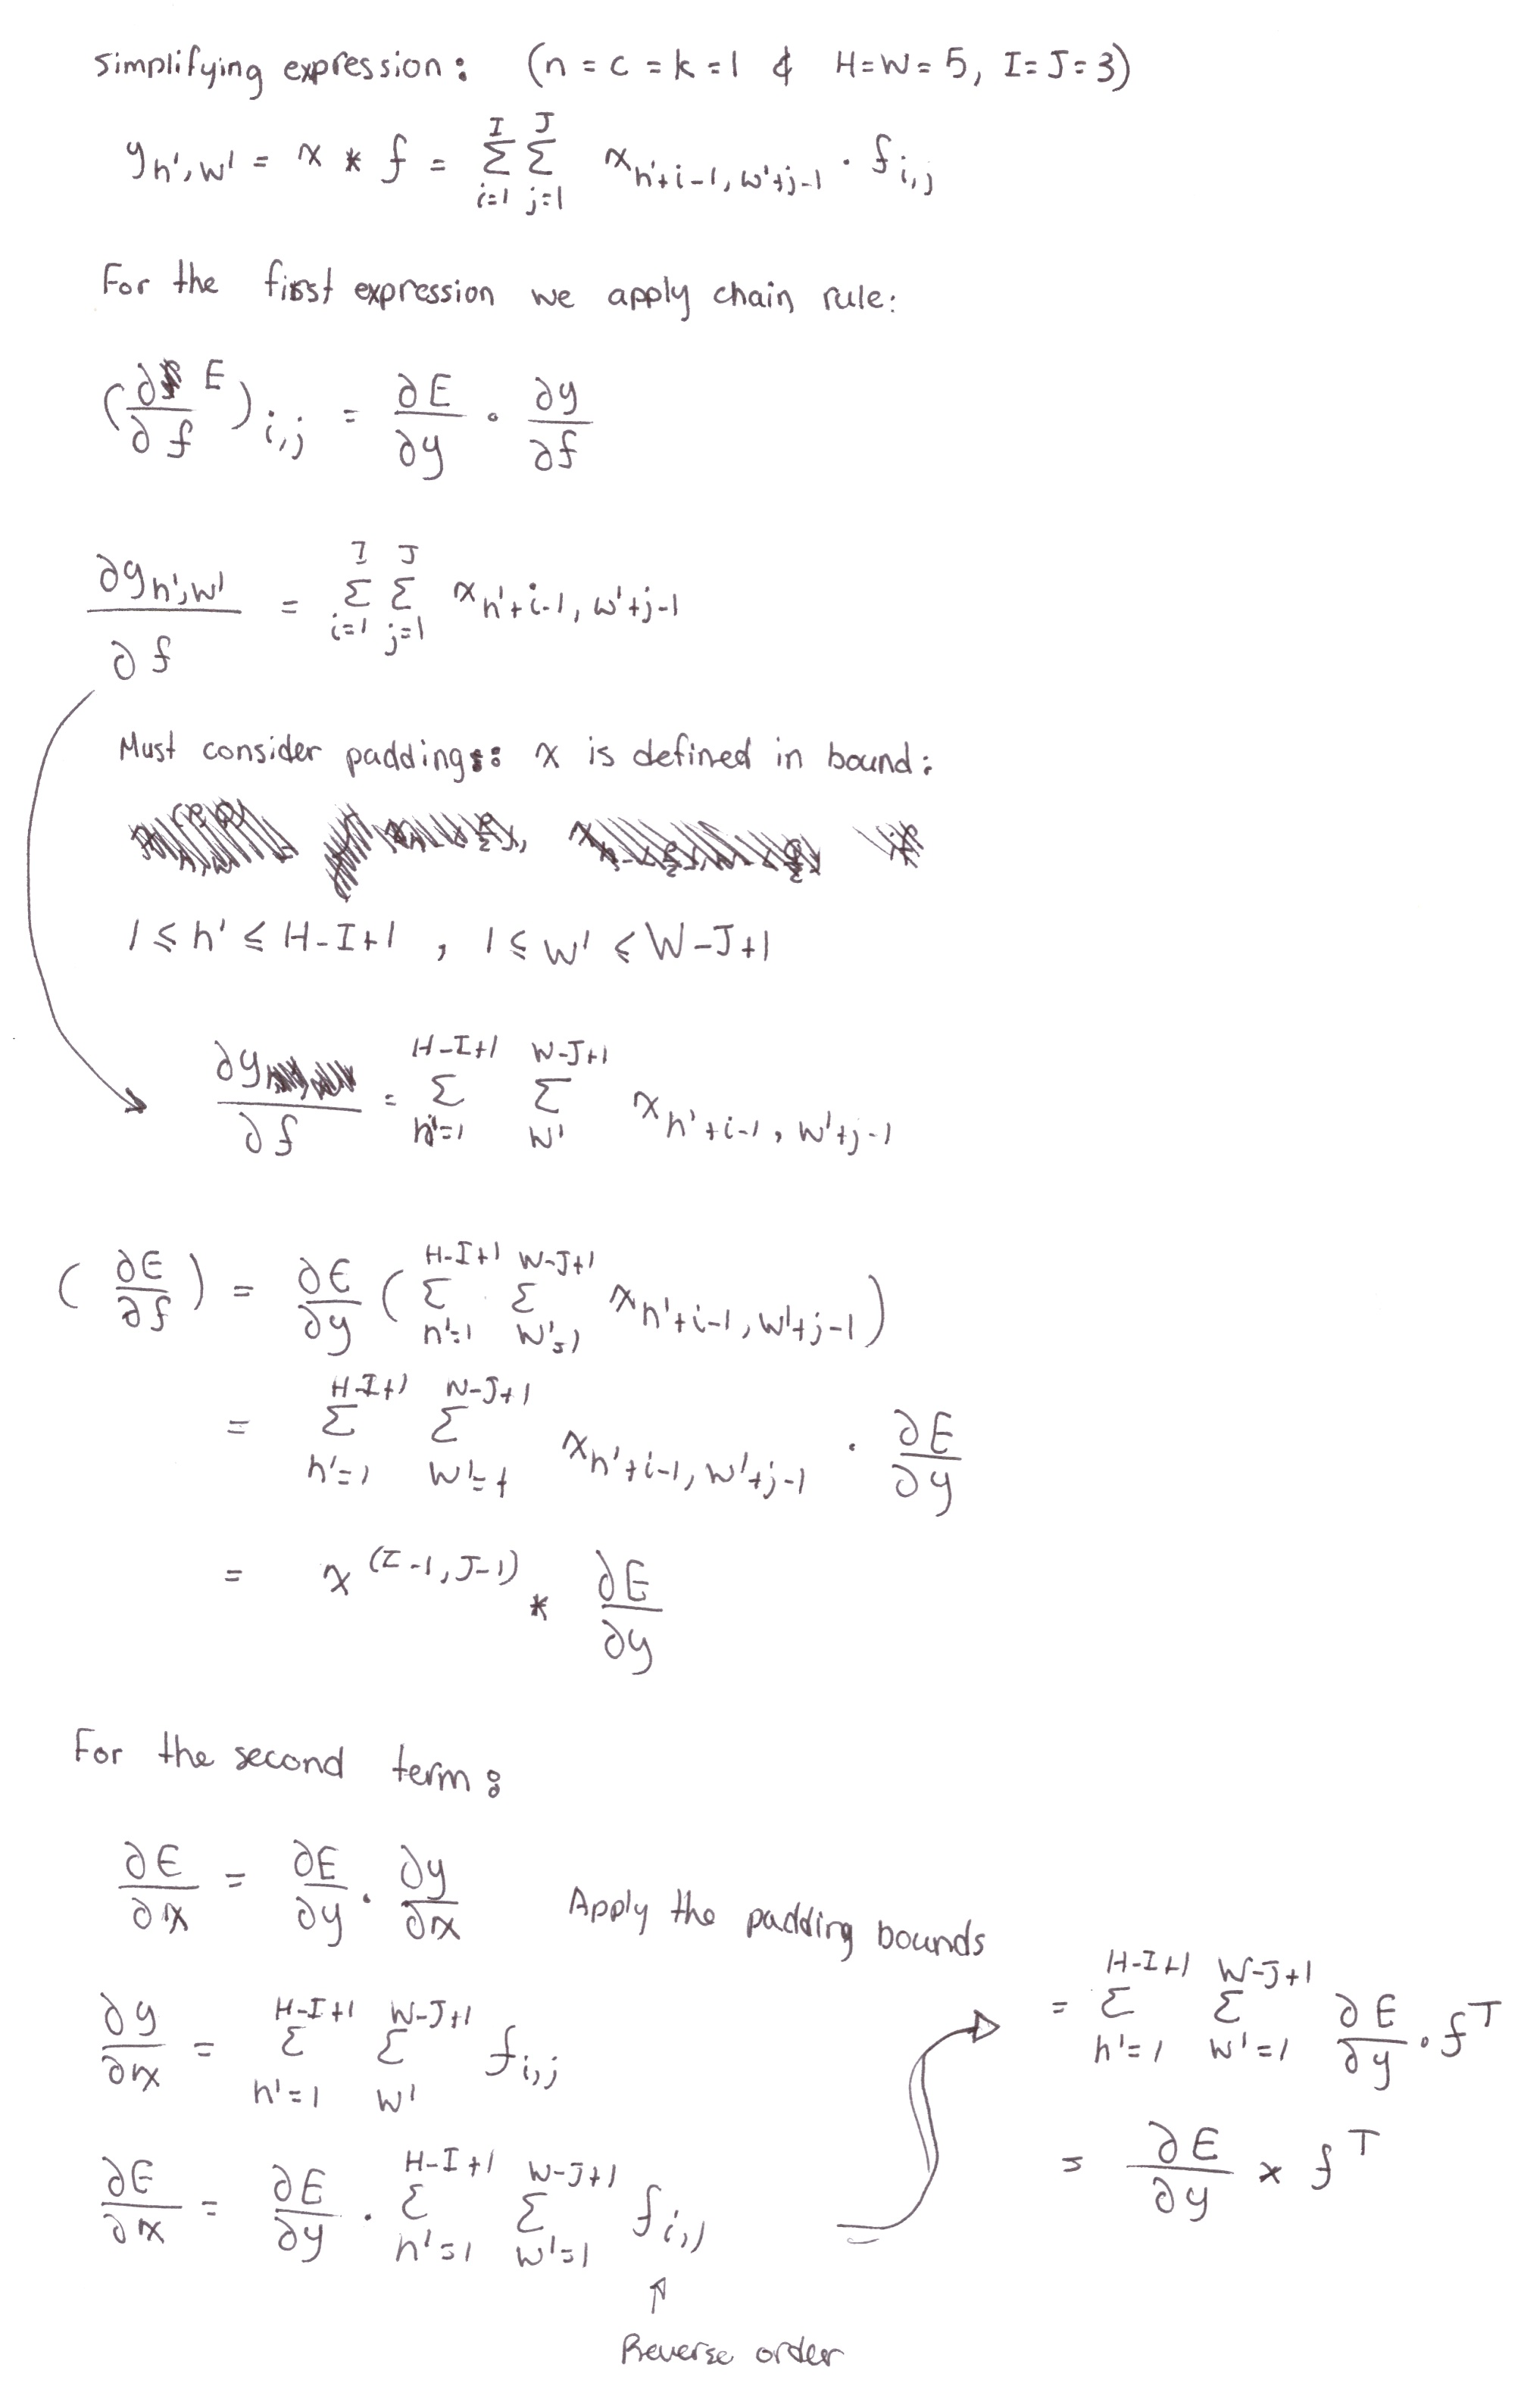
\includegraphics[width=0.7\linewidth]{2/Image.jpg}
\vspace{-0.1in}
\caption{}
\label{f31_a}
\vspace{-0.1in}
\end{figure}

\section{Neural Networks}
\subsection{Basic generalization}

Using the default hyperparameters, both the NN and the CNN were trained. The progression of the accuracy and error for training and validation data in both networks were tracked. Figure \ref{f31_a} shows the accuracy, and Figure \ref{f31_e} shows the error for both NN and CNN. Inspecting both of these figures, we can see similar trends in both networks. The training set is converging to a better accuracy with less error. In NN, the training settles at an accuracy of 0.85625 and error of 0.38740 while the validation set settles at 0.73747 accuracy and 0.95633 error. In CNN, the training set settles at an accuracy of 0.83847 and error of 0.43665 while the validation set settles at 0.79236 accuracy and 0.63323 error. 

In the beginning when the networks have not converged the training set and the validation set have similar accuracy and error. When the networks converge, the parameters are chosen based on the training set hence the offset in both the error and the accuracy is a result of over fitting the parameters to the training set. 

\begin{figure}[!htb]
\centering
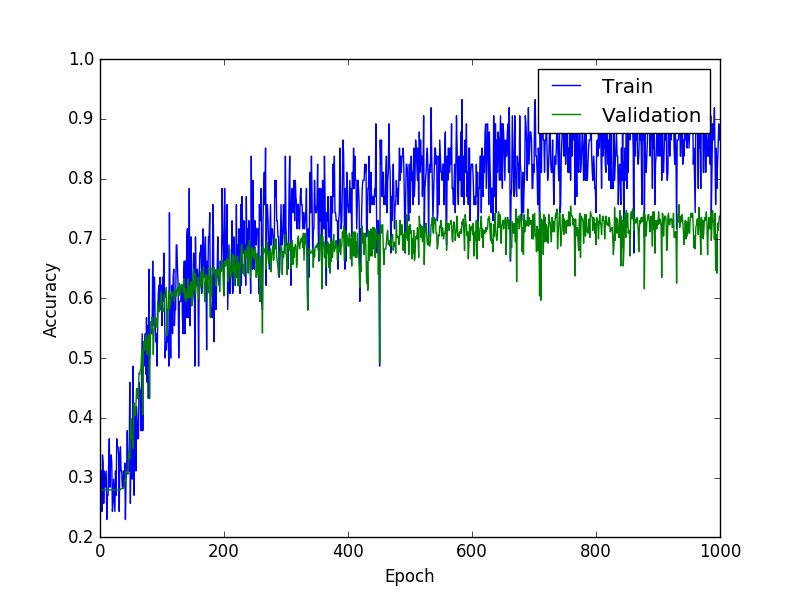
\includegraphics[width=0.4\linewidth]{31/nnA.jpg}
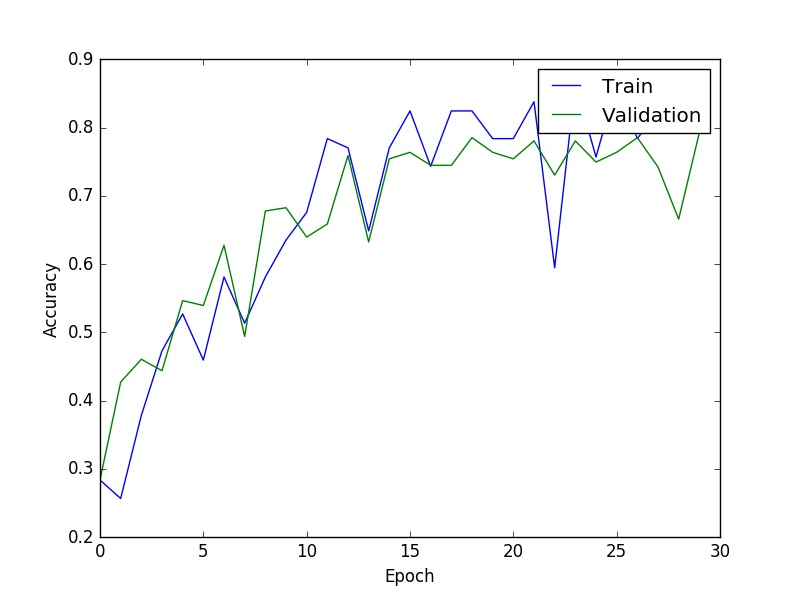
\includegraphics[width=0.4\linewidth]{31/cnnA.jpg}
\vspace{-0.1in}
\caption{Accuracy of training and validation sets for NN (left) and CNN (right).}
\label{f31_a}
\vspace{-0.1in}
\end{figure}

\begin{figure}[!htb]
\centering
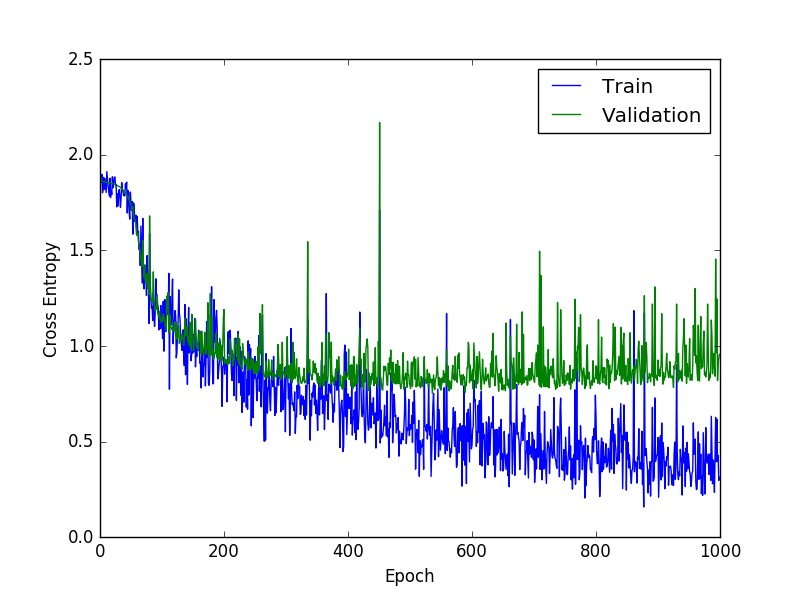
\includegraphics[width=0.4\linewidth]{31/nnE.jpg}
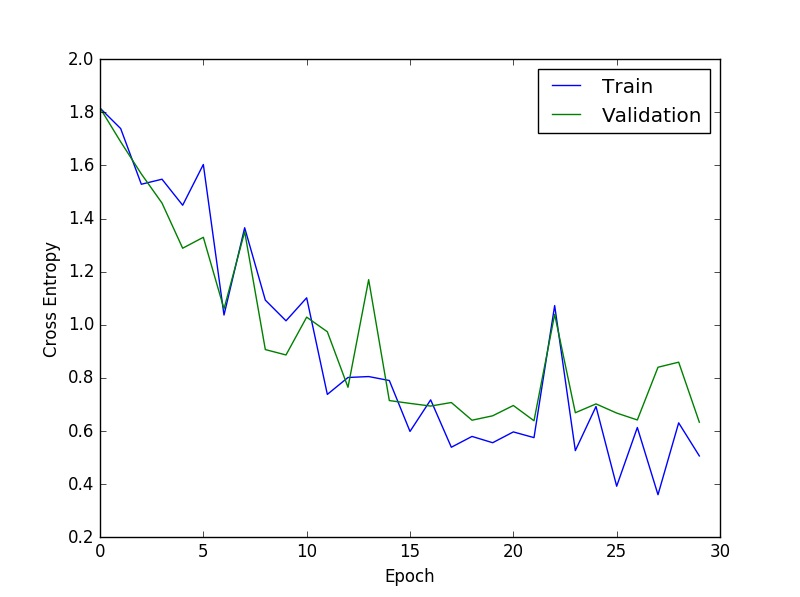
\includegraphics[width=0.4\linewidth]{31/cnnE.jpg}
\vspace{-0.1in}
\caption{Accuracy of training and validation sets for NN (left) and CNN (right).}
\label{f31_e}
\vspace{-0.1in}
\end{figure}

\subsection{Optimization}
\subsubsection*{Learning Rate}
For this section the learning rate $\epsilon$ of 0.001, 0.01, 0.05, 0.1, and 1.0 are used. An additional learning rate of 0.005 is used for NN to gain better understanding of the accuracy and error trend. Inspecting the plots of accuracy and errors of the mentioned learning rates, it is easily distinguishable that some values outperform the rest. The plot for accuracy and error plots for the learning rates of 0.001, 0.01, 0.1, and 1.0 can be found in Figure \ref{f32_a} and Figure \ref{f32_e}. From these plots it is evident and the learning rate parameter effected the convergence of both networks. For both networks, the learning rates of 0.001, 0.005, and 1.0 can be ignored as they are either too low or too high, causing the network to converge very slowly or not at all. To better understand what is the optimal learning rate, Figure \ref{f32} was used to see to what accuracy and error did each rates converge to. For NN, the learning rate of 0.05 resulted in the best accuracy for both the training set and the validation set. Moreover, for this rate, the error was also the lowest for both sets. For CNN, the learning rate of 0.1 resulted in the best accuracy and the lowest error for both the training and validation set.  

\begin{figure}[!htb]
\centering
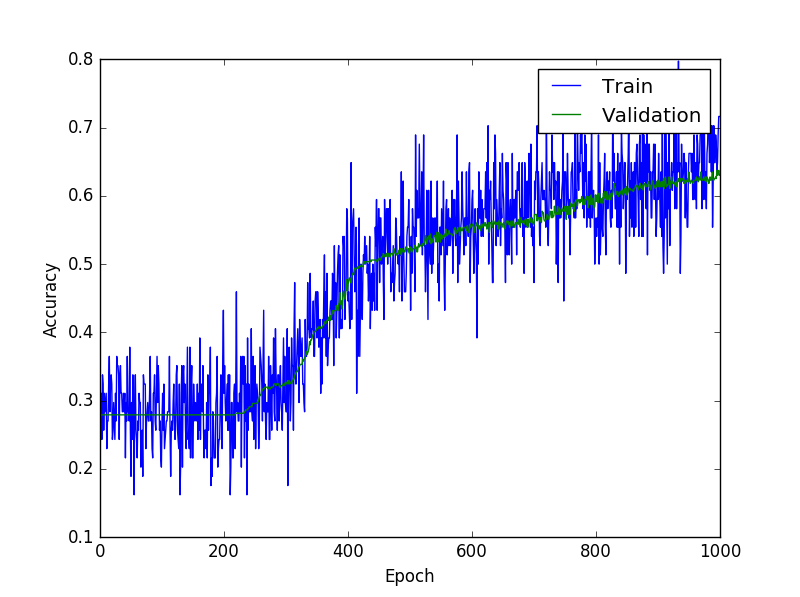
\includegraphics[width=0.23\linewidth]{32/eps/nn/0001A.png}
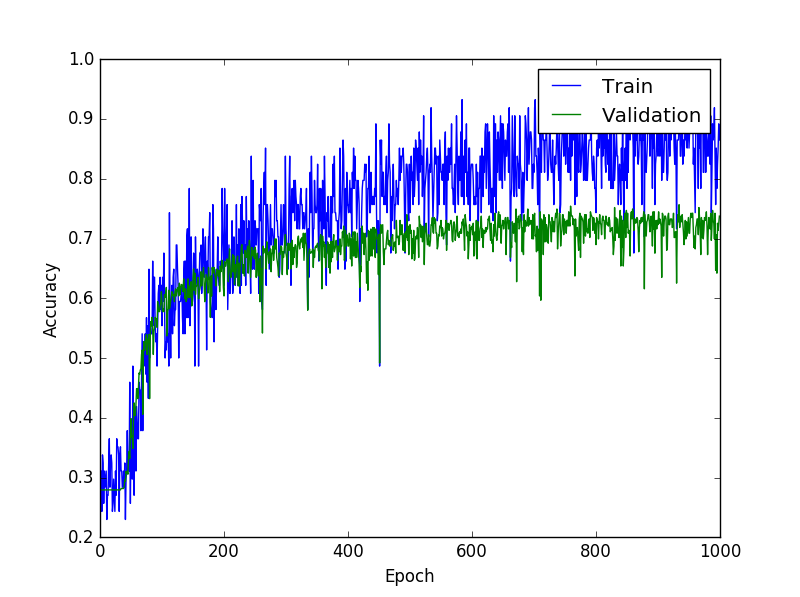
\includegraphics[width=0.23\linewidth]{32/eps/nn/001A.png}
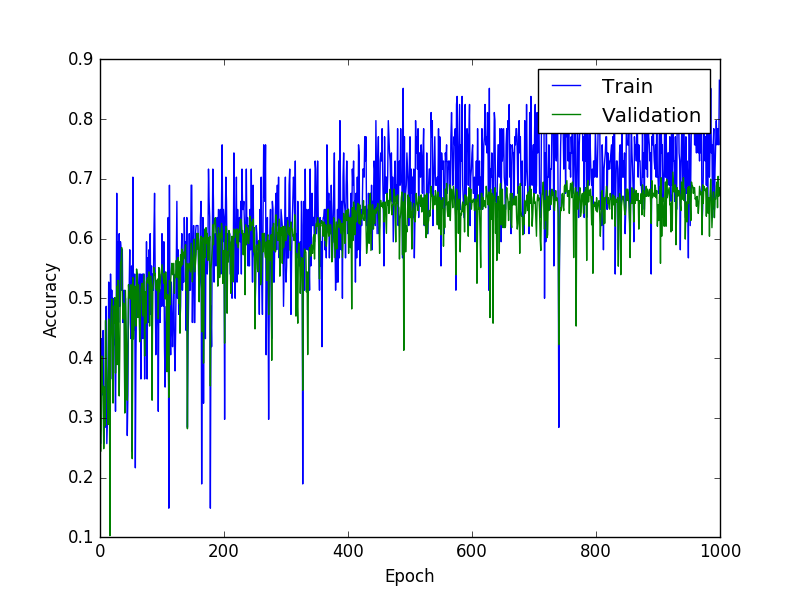
\includegraphics[width=0.23\linewidth]{32/eps/nn/01A.png}
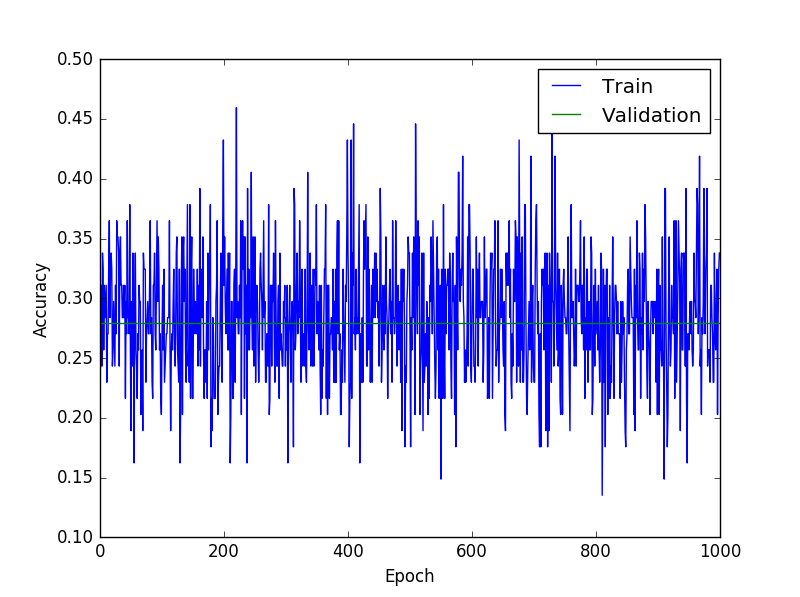
\includegraphics[width=0.23\linewidth]{32/eps/nn/1A.png}

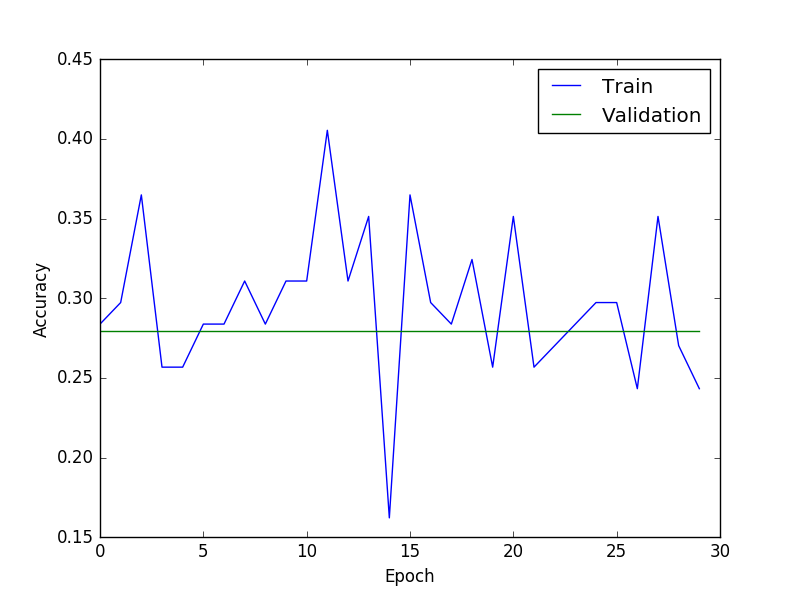
\includegraphics[width=0.23\linewidth]{32/eps/cnn/0001A.png}
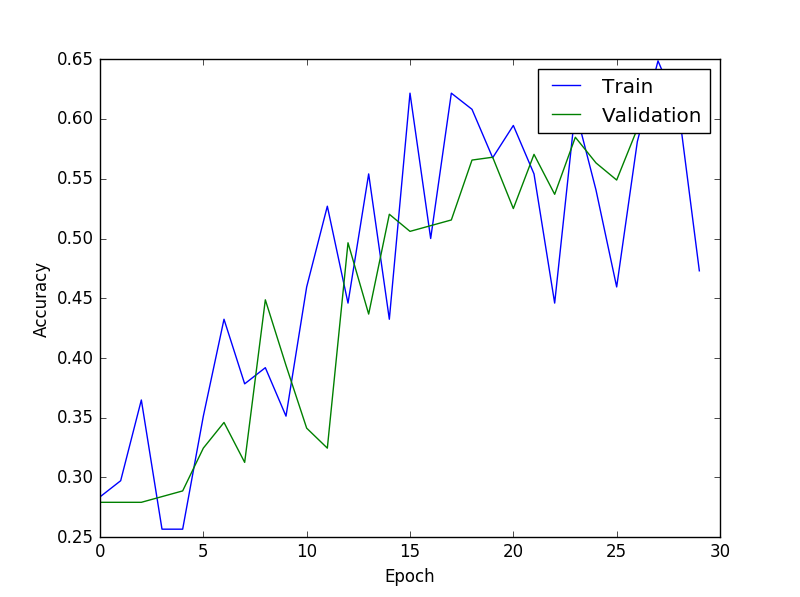
\includegraphics[width=0.23\linewidth]{32/eps/cnn/001A.png}
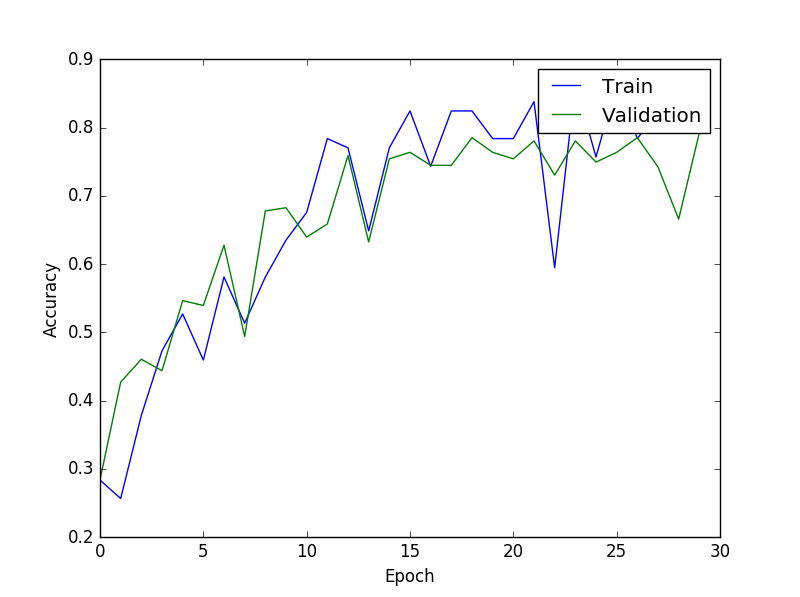
\includegraphics[width=0.23\linewidth]{32/eps/cnn/01A.png}
\includegraphics[width=0.23\linewidth]{32/eps/cnn/1A.png}

\vspace{-0.1in}
\caption{Accuracy of different learning rates(Left to right: 0.001, 0.01, 0.1, 1.0), NN (top) and CNN (bottom).}
\label{f32_a}
\vspace{-0.1in}
\end{figure}

\begin{figure}[!htb]
\centering
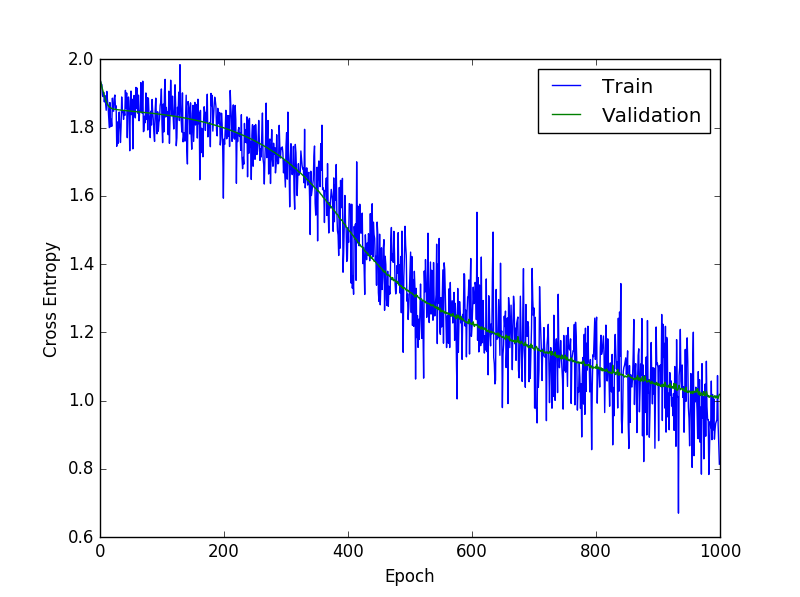
\includegraphics[width=0.23\linewidth]{32/eps/nn/0001E.png}
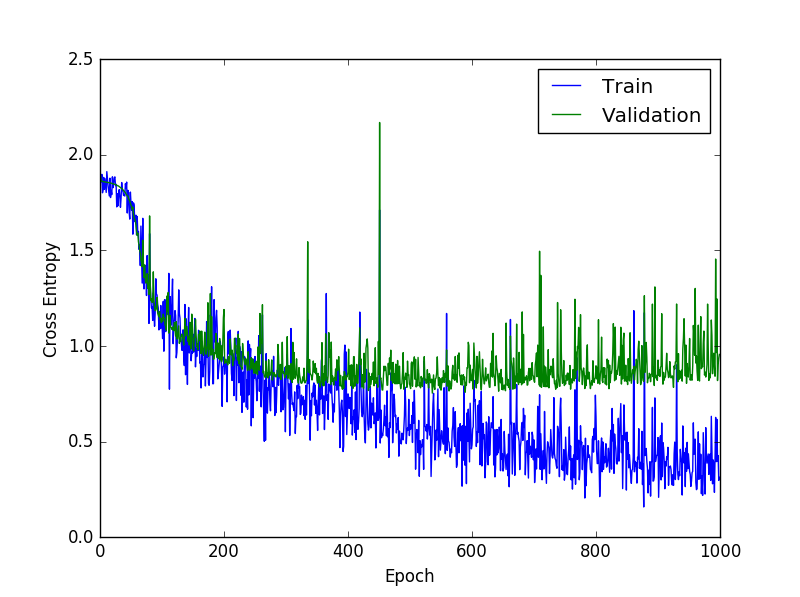
\includegraphics[width=0.23\linewidth]{32/eps/nn/001E.png}
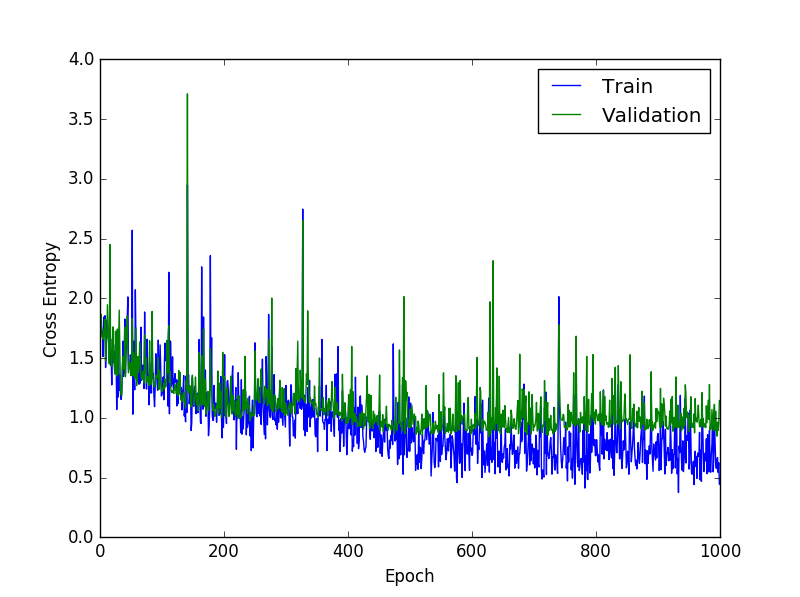
\includegraphics[width=0.23\linewidth]{32/eps/nn/01E.png}
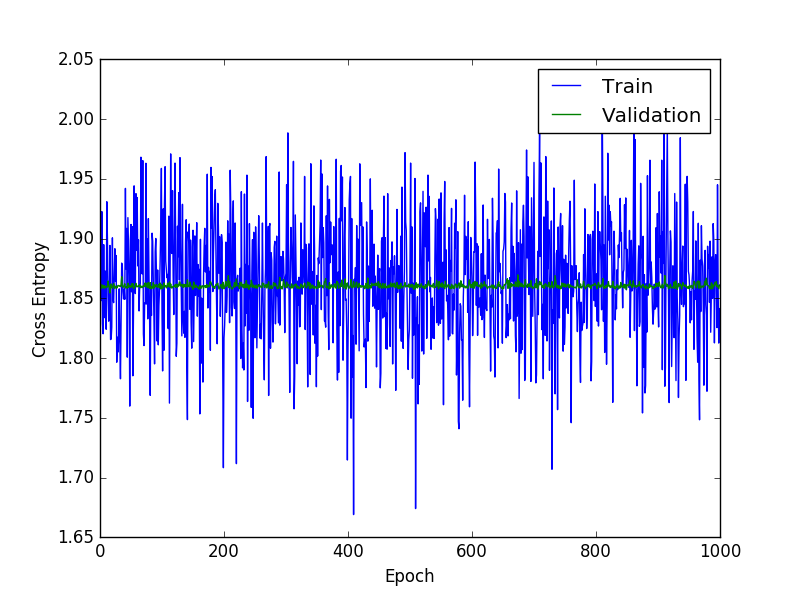
\includegraphics[width=0.23\linewidth]{32/eps/nn/1E.png}

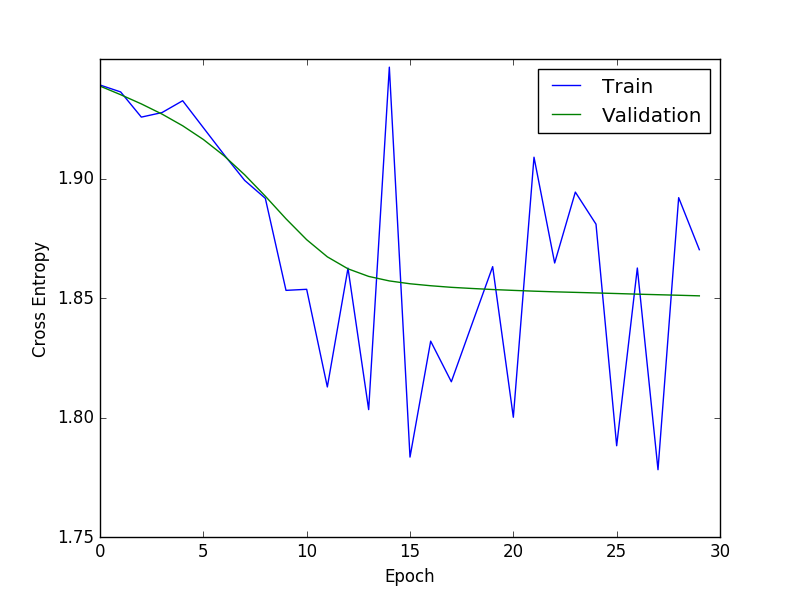
\includegraphics[width=0.23\linewidth]{32/eps/cnn/0001E.png}
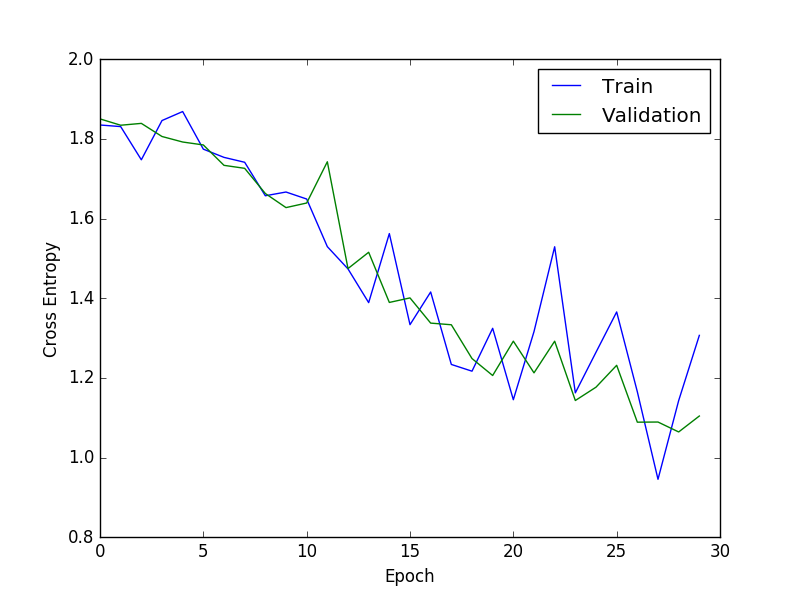
\includegraphics[width=0.23\linewidth]{32/eps/cnn/001E.png}
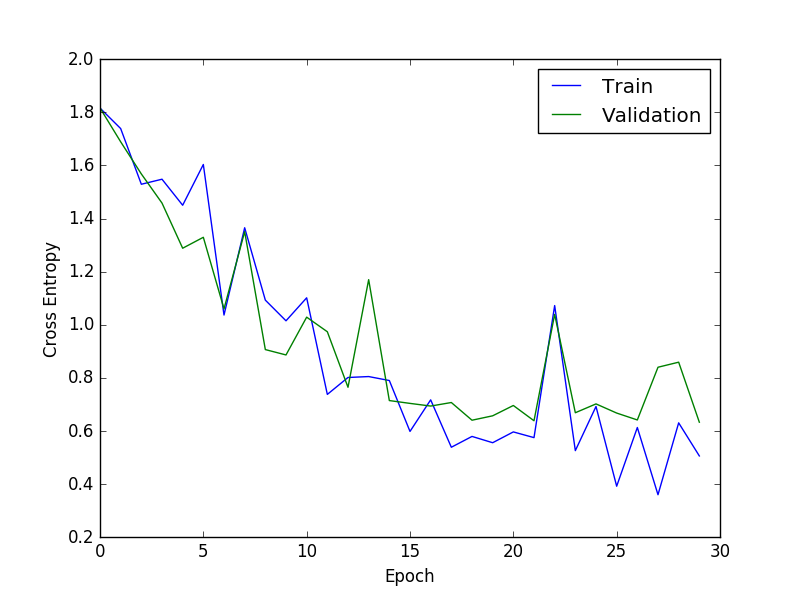
\includegraphics[width=0.23\linewidth]{32/eps/cnn/01E.png}
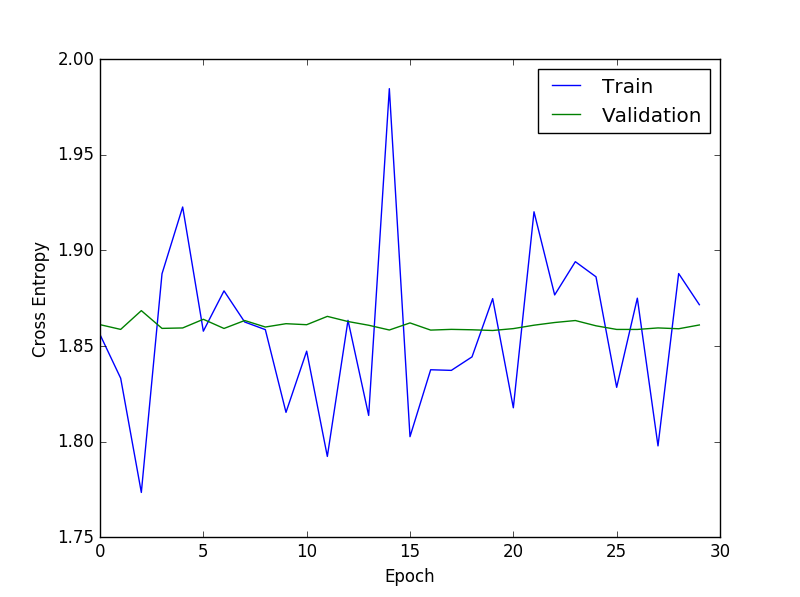
\includegraphics[width=0.23\linewidth]{32/eps/cnn/1E.png}

\vspace{-0.1in}
\caption{Error of different learning rates(Left to right: 0.001, 0.01, 0.1, 1.0), NN (top) and CNN (bottom).}
\label{f32_e}
\vspace{-0.1in}
\end{figure}

\begin{figure}[!htb]
\centering
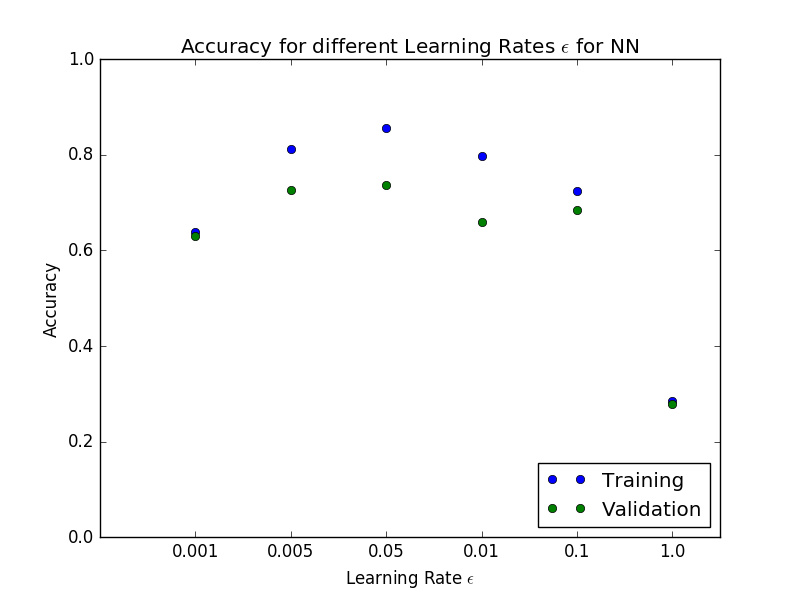
\includegraphics[width=0.4\linewidth]{32/eps/nn/Accuracy.png}
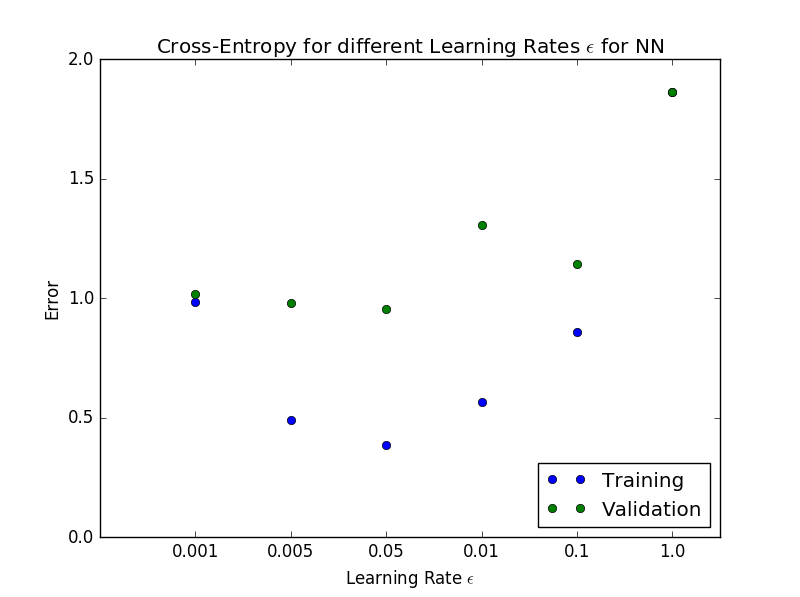
\includegraphics[width=0.4\linewidth]{32/eps/nn/Error.png}
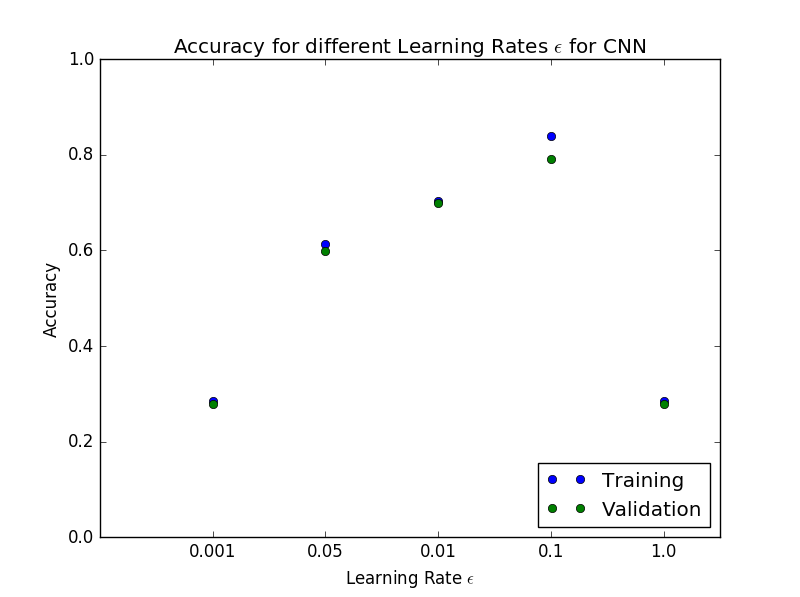
\includegraphics[width=0.4\linewidth]{32/eps/cnn/Accuracy.png}
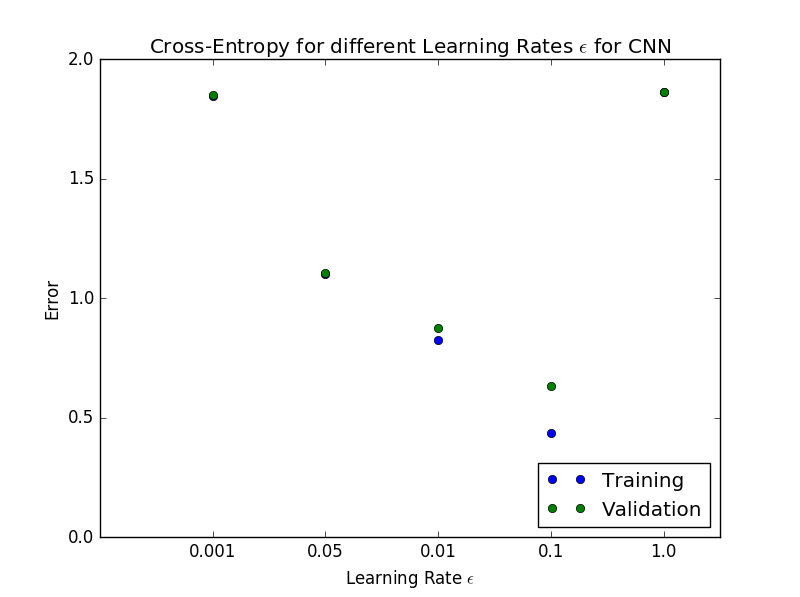
\includegraphics[width=0.4\linewidth]{32/eps/cnn/Error.png}
\vspace{-0.1in}
\caption{Converged accuracy and error for different learning rates, NN (top) and CNN (bottom).}
\label{f32}
\vspace{-0.1in}
\end{figure}

\subsubsection*{Momentum}
To see the effect of momentum on the convergence rate, the momentum values of 0.3, 0.6, 0.9 are used. The default momentum value of 0.0 is also included to gain more insight on the effect of momentum. Figure \ref{f32_ma} and Figure \ref{f32_me} contain the plots of the accuracy and error for all momentums. The purpose of adding momentum to the system is to attenuate the oscillation in the gradient decent. From both figures, it can be seen that momentum value of 0.0 values there is a lot of oscillation, but at values of 0.3 and 0.6 the oscillation has diminished. At 0.9 the momentum starts to interfere with the gradient decent and the system has become unstable. Therefore, momentum helps the network to converge to a more stable accuracy and error value. From Figure \ref{f32m}, it can be said that both the momentum of 0.6 slightly outperform the value of 0.3 in terms of better accuracy and less error for both NN and CNN.  

\begin{figure}[!htb]
\centering
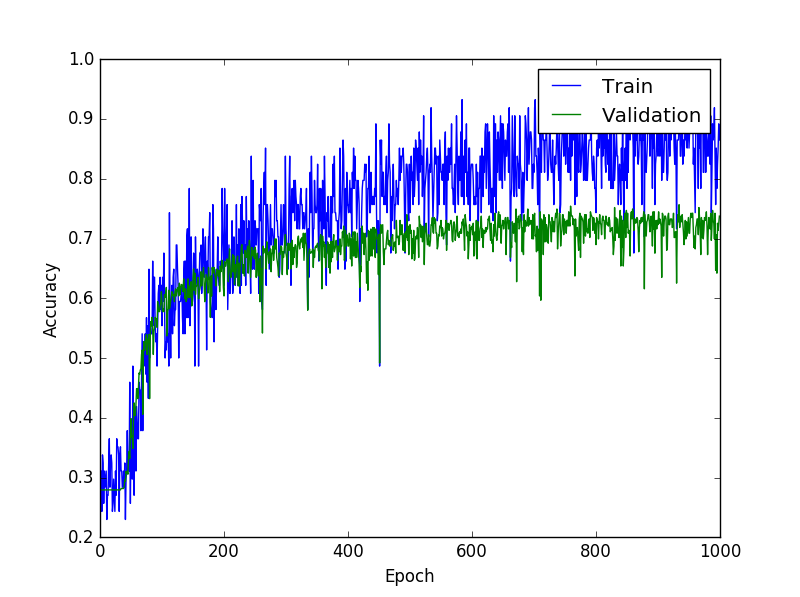
\includegraphics[width=0.23\linewidth]{32/mom/nn/00A.png}
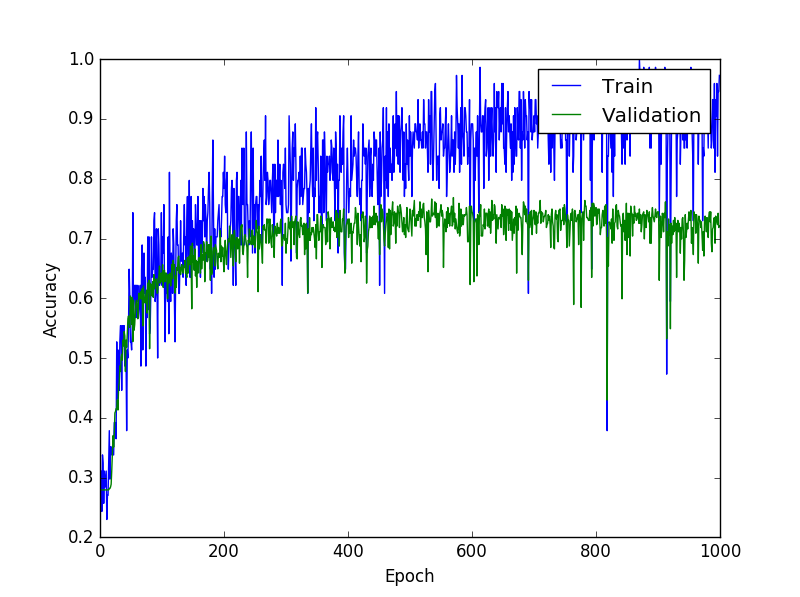
\includegraphics[width=0.23\linewidth]{32/mom/nn/03A.png}
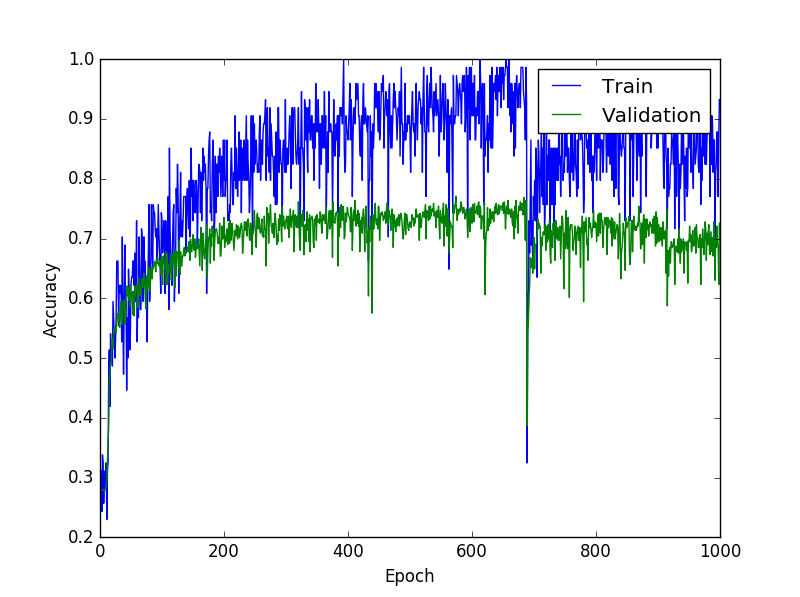
\includegraphics[width=0.23\linewidth]{32/mom/nn/06A.png}
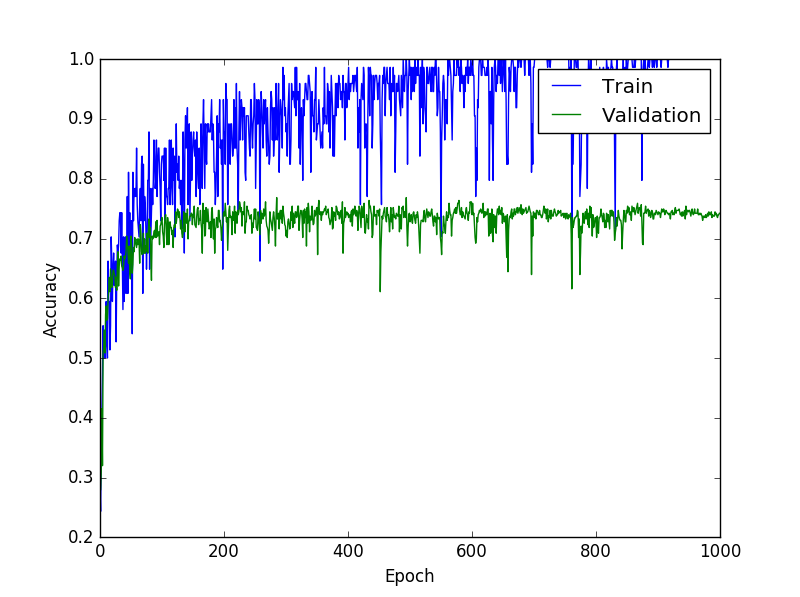
\includegraphics[width=0.23\linewidth]{32/mom/nn/09A.png}

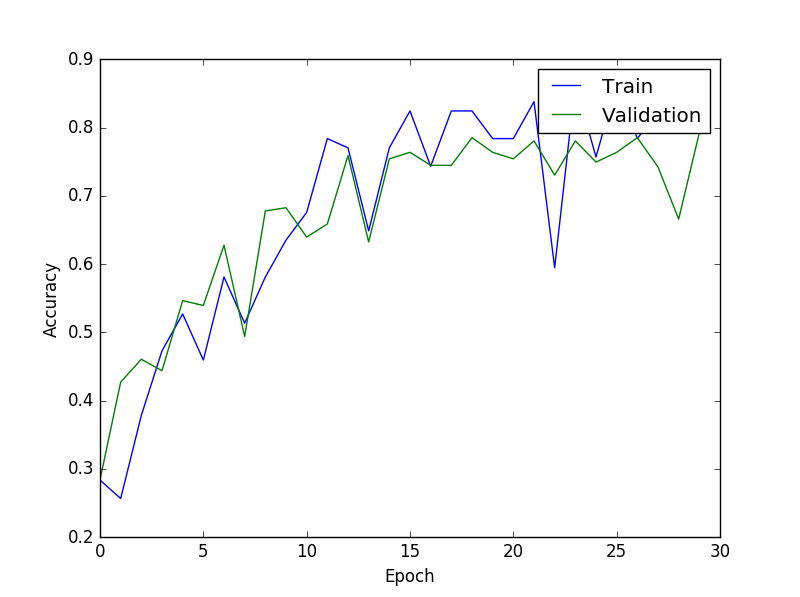
\includegraphics[width=0.23\linewidth]{32/mom/cnn/00A.png}
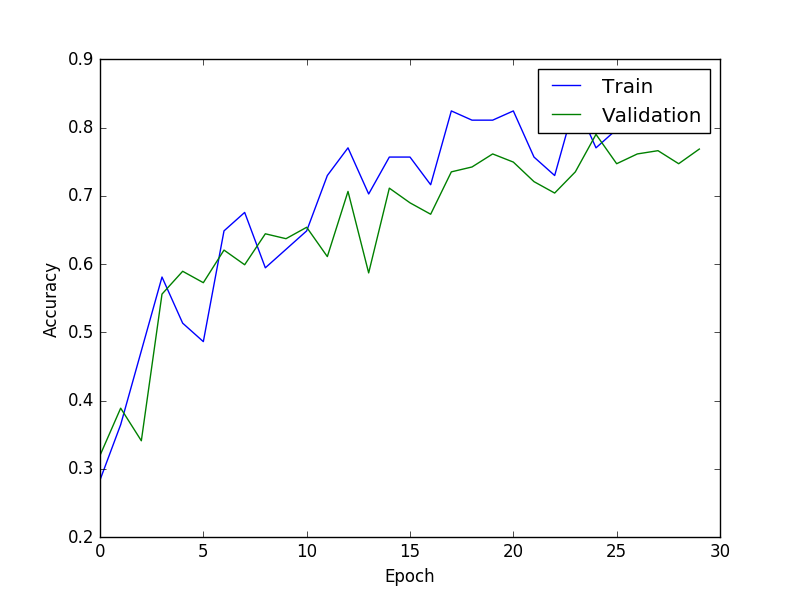
\includegraphics[width=0.23\linewidth]{32/mom/cnn/03A.png}
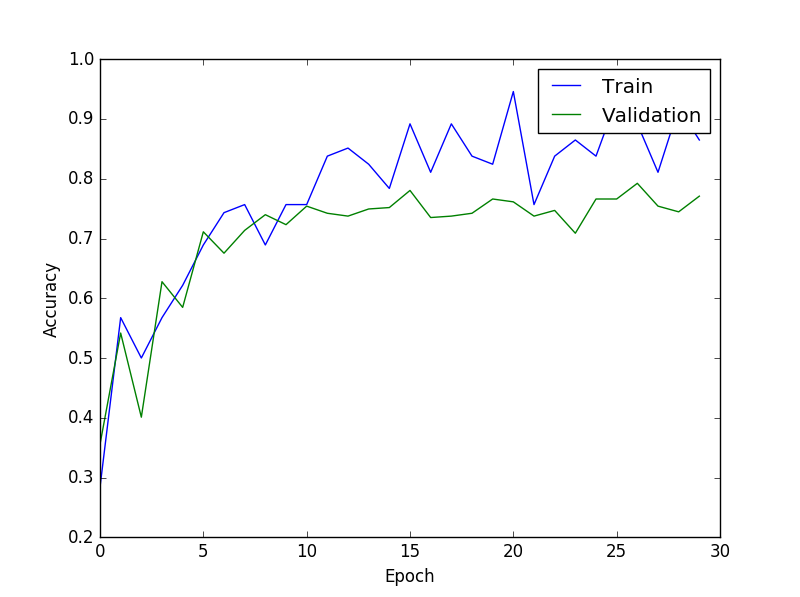
\includegraphics[width=0.23\linewidth]{32/mom/cnn/06A.png}
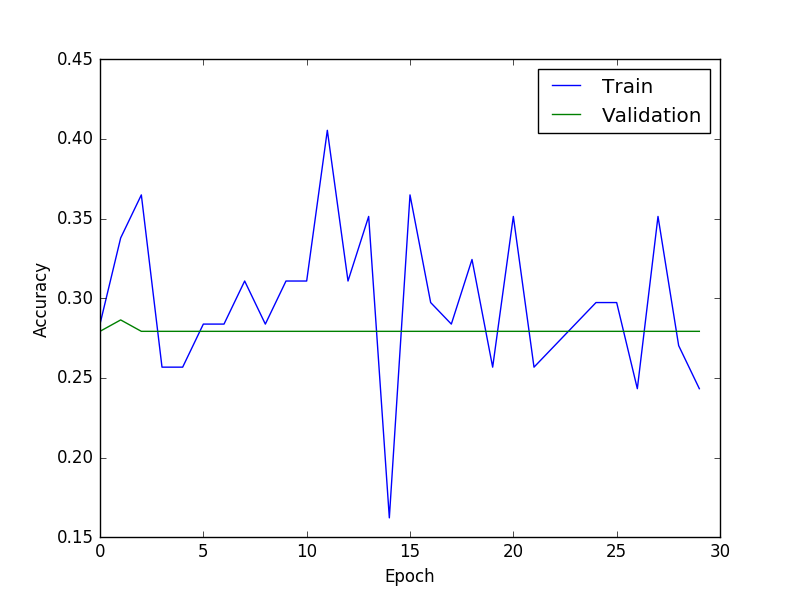
\includegraphics[width=0.23\linewidth]{32/mom/cnn/09A.png}

\vspace{-0.1in}
\caption{Accuracy of different momentums (Left to right: 0.0, 0.3, 0.6, 0.9), NN (top) and CNN (bottom).}
\label{f32_ma}
\vspace{-0.1in}
\end{figure}

\begin{figure}[!htb]
\centering
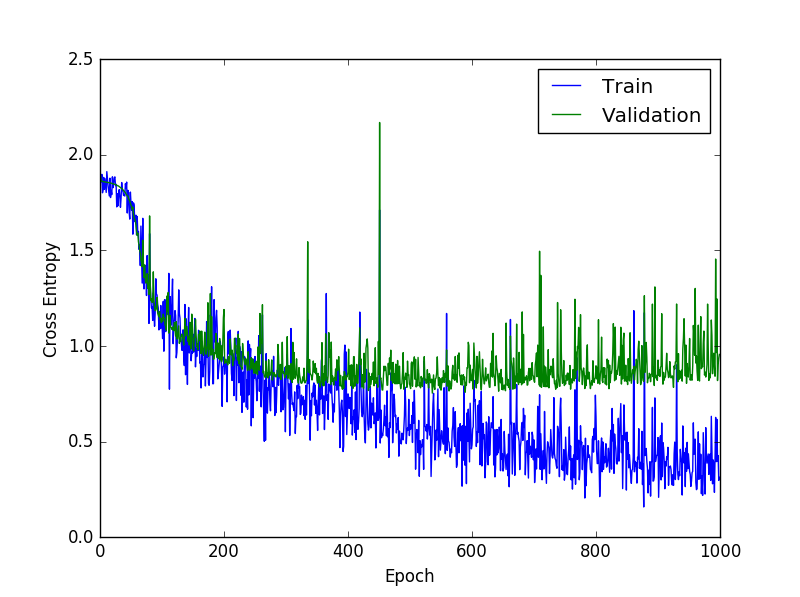
\includegraphics[width=0.23\linewidth]{32/mom/nn/00E.png}
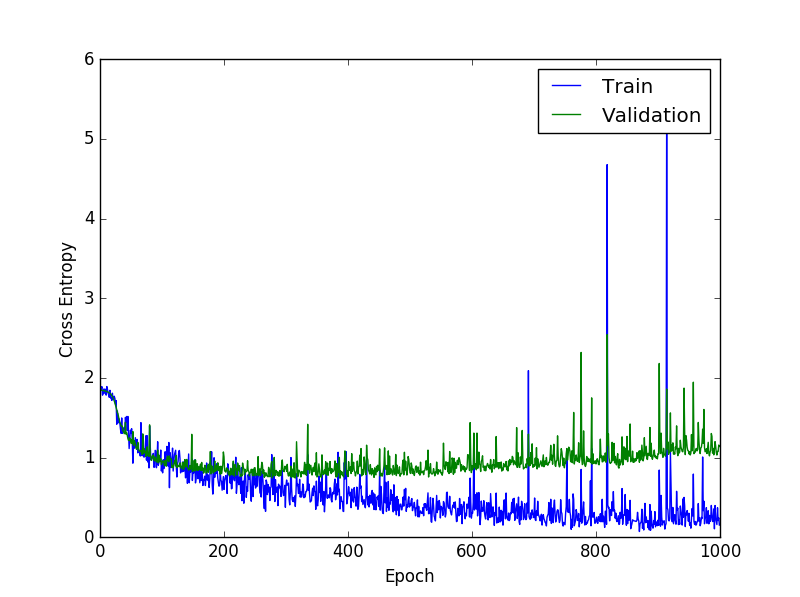
\includegraphics[width=0.23\linewidth]{32/mom/nn/03E.png}
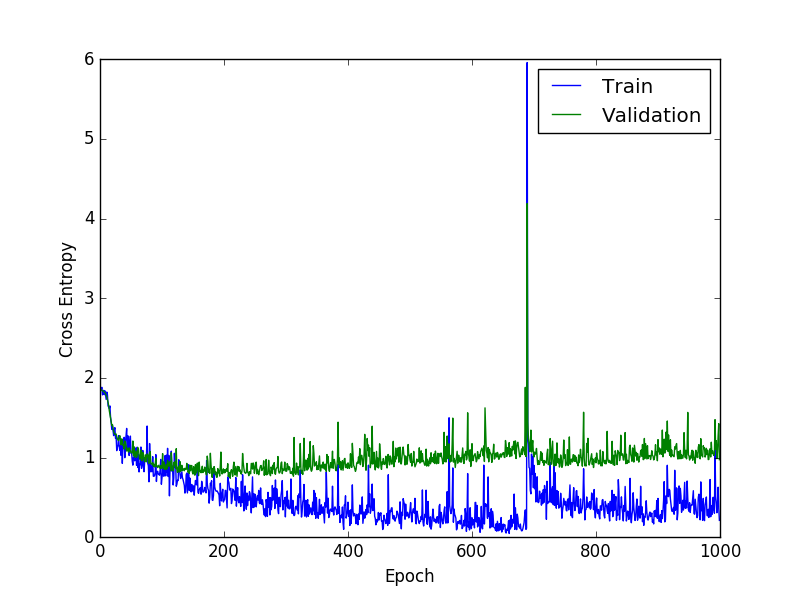
\includegraphics[width=0.23\linewidth]{32/mom/nn/06E.png}
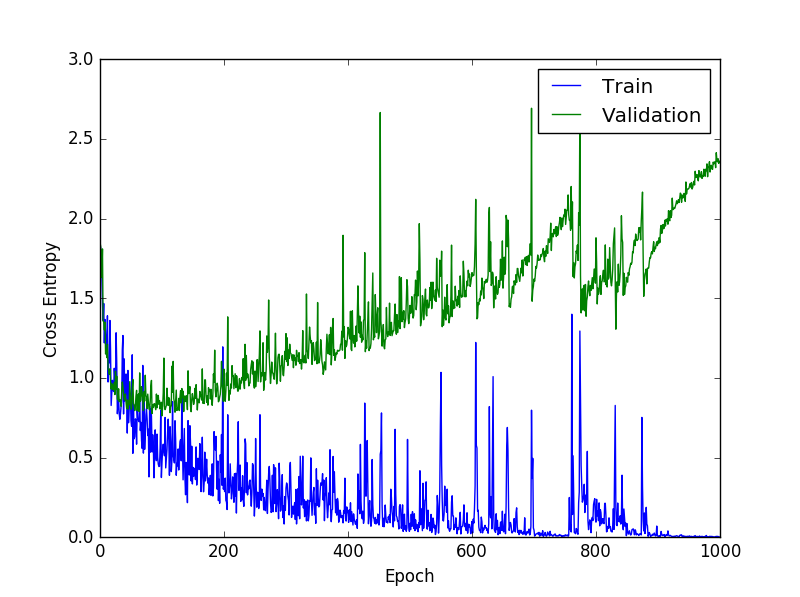
\includegraphics[width=0.23\linewidth]{32/mom/nn/09E.png}

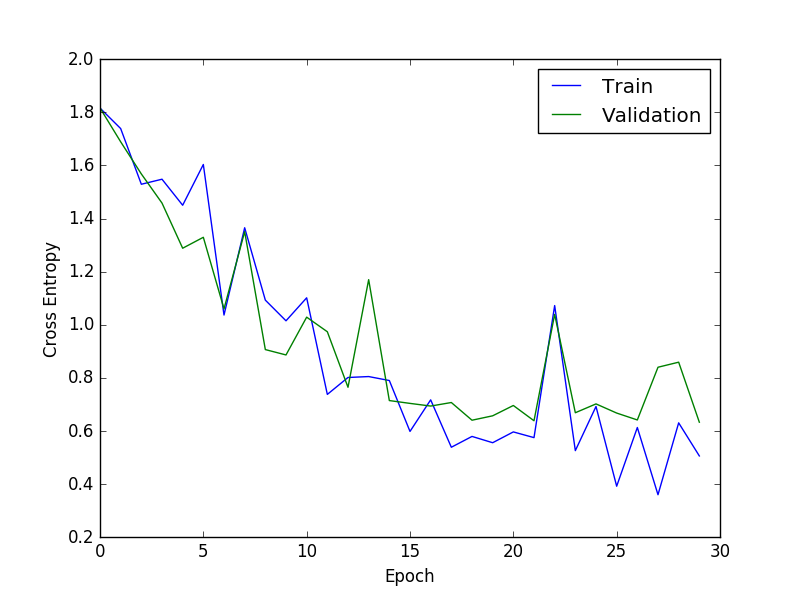
\includegraphics[width=0.23\linewidth]{32/mom/cnn/00E.png}
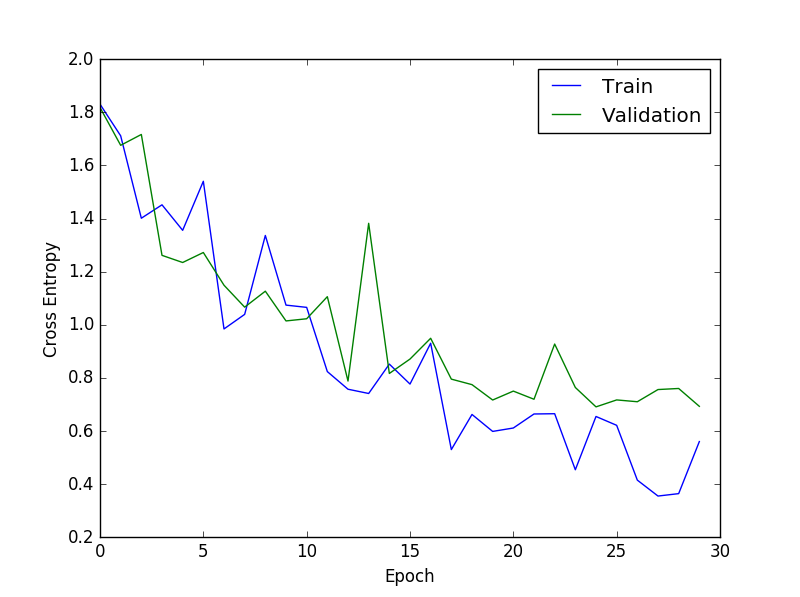
\includegraphics[width=0.23\linewidth]{32/mom/cnn/03E.png}
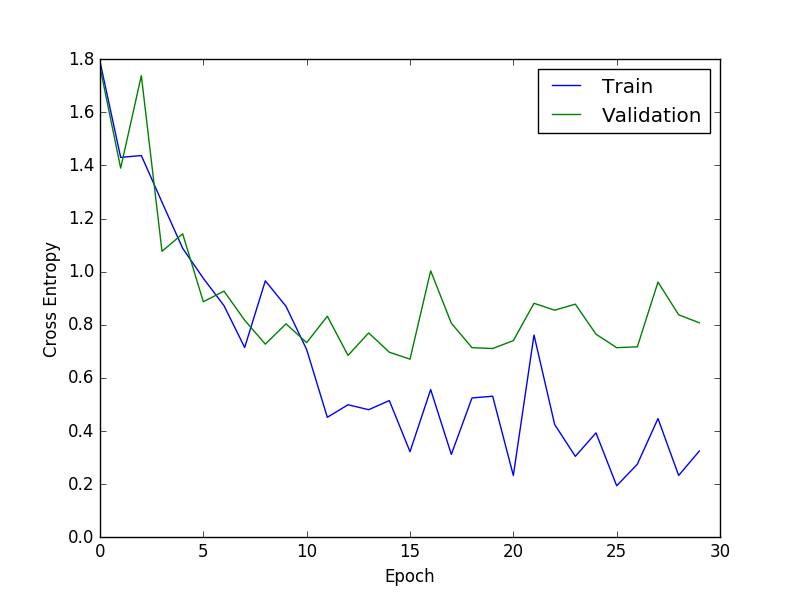
\includegraphics[width=0.23\linewidth]{32/mom/cnn/06E.png}
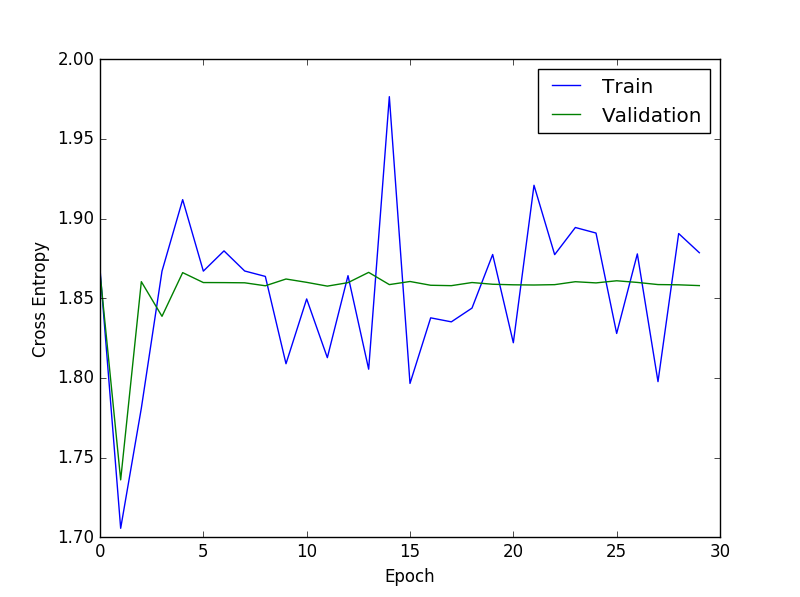
\includegraphics[width=0.23\linewidth]{32/mom/cnn/09E.png}

\vspace{-0.1in}
\caption{Error of different momentums (Left to right: 0.0, 0.3, 0.6, 0.9), NN (top) and CNN (bottom).}
\label{f32_me}
\vspace{-0.1in}
\end{figure}

\begin{figure}[!htb]
\centering
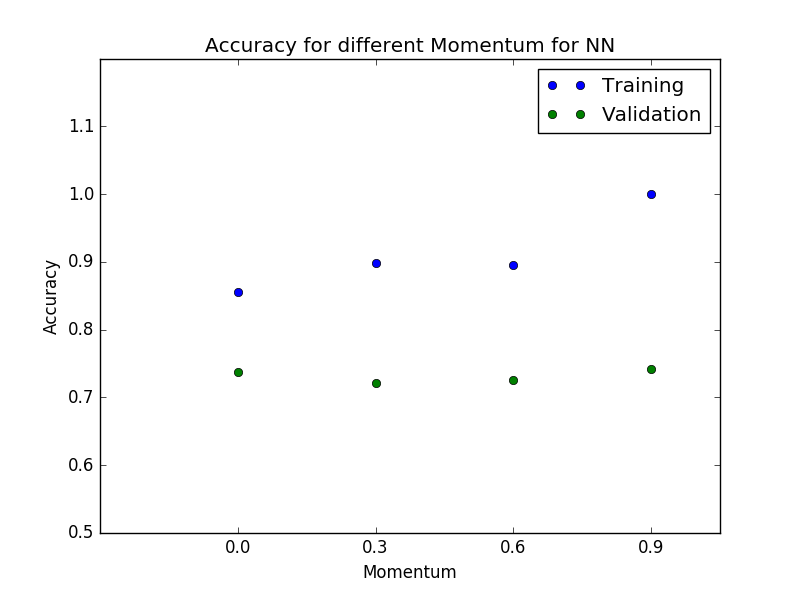
\includegraphics[width=0.4\linewidth]{32/mom/nn/Accuracy.png}
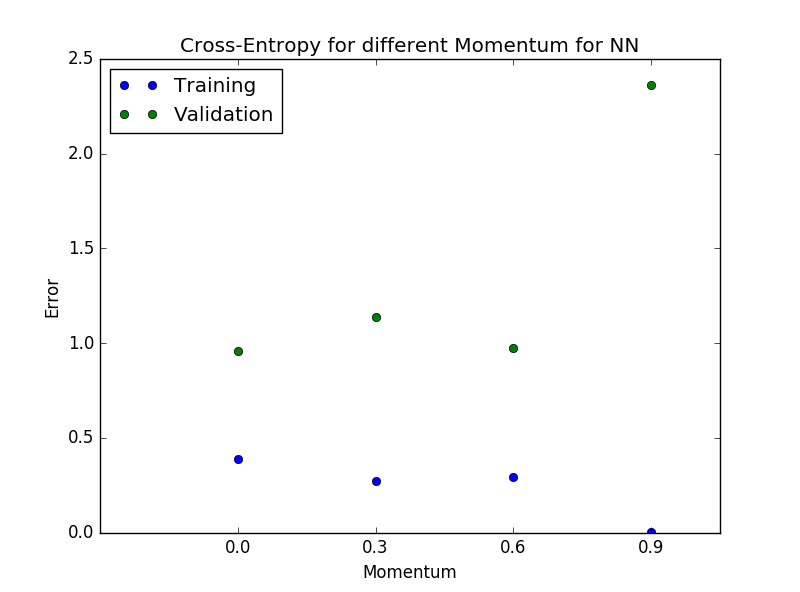
\includegraphics[width=0.4\linewidth]{32/mom/nn/Error.png}
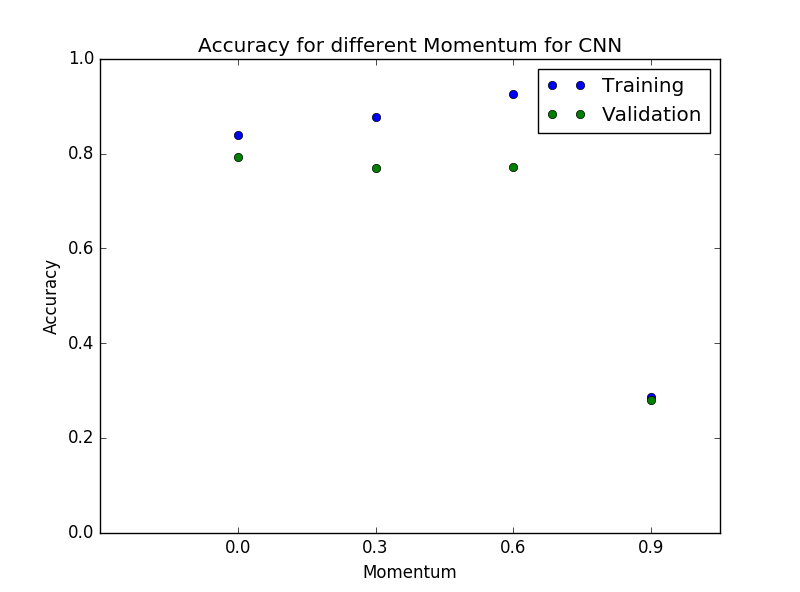
\includegraphics[width=0.4\linewidth]{32/mom/cnn/Accuracy.png}
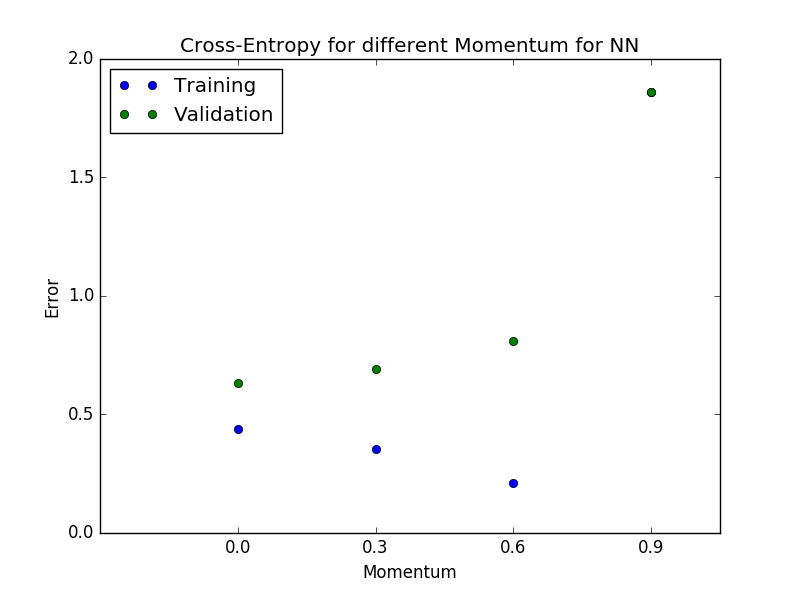
\includegraphics[width=0.4\linewidth]{32/mom/cnn/Error.png}
\vspace{-0.1in}
\caption{Converged accuracy and error for different momentums, NN (top) and CNN (bottom).}
\label{f32m}
\vspace{-0.1in}
\end{figure}

\subsubsection*{Batch Size}
For this section, batch sized of 1, 10, 100, 500, and 1000 are used. Figure \ref{f32_ba} and Figure \ref{f32_be} contain the plots of the accuracy and error for all of the different batch sizes. In both NN and CNN it can be seen that batch sizes of 1 and 10 are not sufficient in making the model converge. For batch size of 100, the model converges but now it is over fitting the training set. For 500, the model converges slower than 100 but it has less bias in NN and its less stable in CNN. Batch size of 1000 has even a slower convergence rate than 500 in NN, and for CNN it never converges. To decide if a batch size of 100 or 500 is suitable we inspect Figure \ref{f32b}. In NN, batch size of 100 has better accuracy for both training and validation set, and it has less error for the training set but not the validation set. In CNN, batch size of 100 is superior to 500 in both accuracy and error in both training and validation set. Therefore, for both network the best batch size is 100.  
  
\begin{figure}[!htb]
\centering
\includegraphics[width=0.18\linewidth]{32/batch/nn/1A.png}
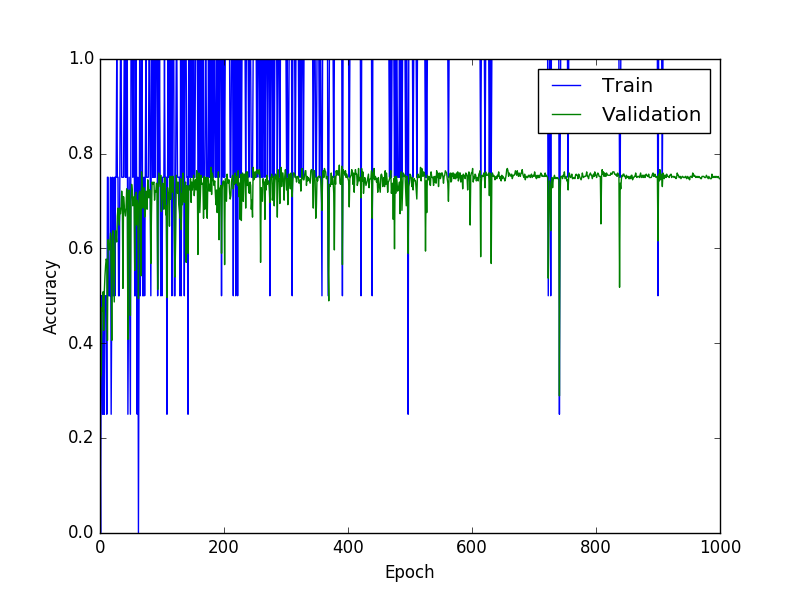
\includegraphics[width=0.18\linewidth]{32/batch/nn/10A.png}
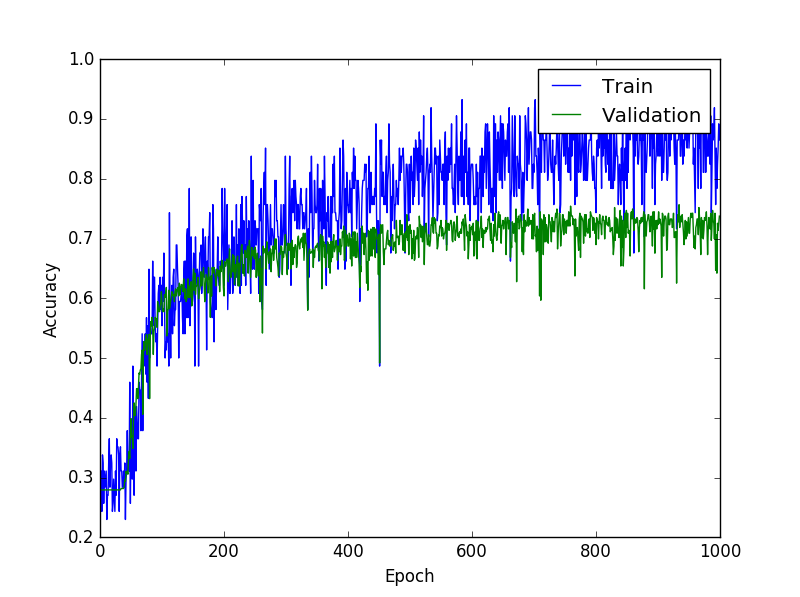
\includegraphics[width=0.18\linewidth]{32/batch/nn/100A.png}
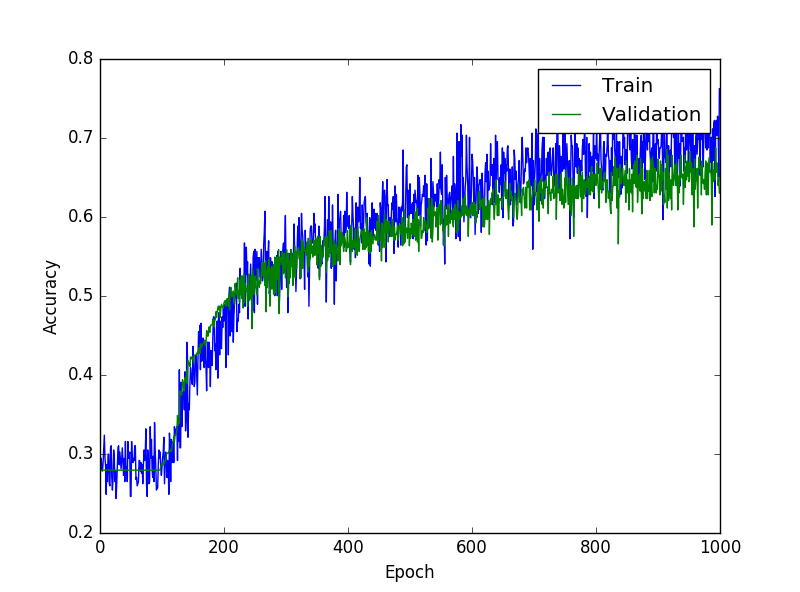
\includegraphics[width=0.18\linewidth]{32/batch/nn/500A.png}
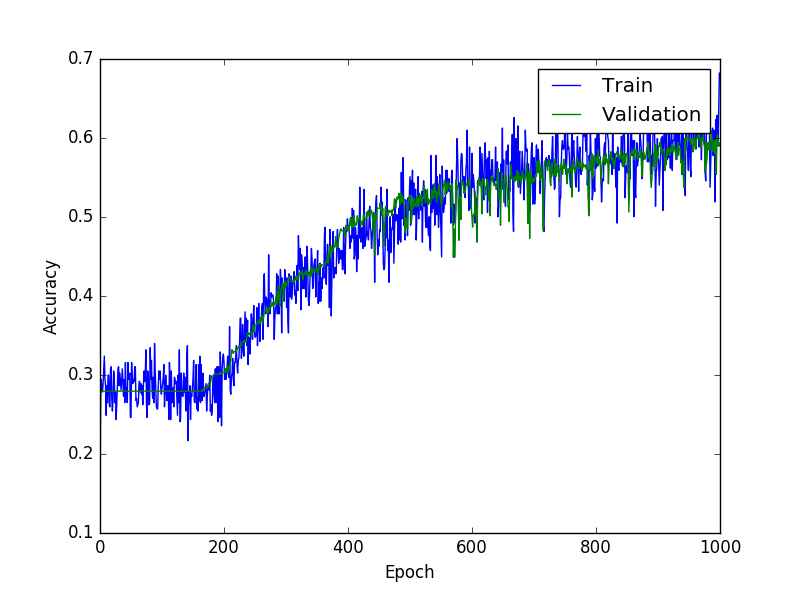
\includegraphics[width=0.18\linewidth]{32/batch/nn/1000A.png}

\includegraphics[width=0.18\linewidth]{32/batch/cnn/1A.png}
\includegraphics[width=0.18\linewidth]{32/batch/cnn/10A.png}
\includegraphics[width=0.18\linewidth]{32/batch/cnn/100A.png}
\includegraphics[width=0.18\linewidth]{32/batch/cnn/500A.png}
\includegraphics[width=0.18\linewidth]{32/batch/cnn/1000A.png}

\vspace{-0.1in}
\caption{Accuracy of different batch sizes (Left to right: 1, 10, 100, 500, 1000), NN (top) and CNN (bottom).}
\label{f32_ba}
\vspace{-0.1in}
\end{figure}

\begin{figure}[!htb]
\centering
\includegraphics[width=0.18\linewidth]{32/batch/nn/1E.png}
\includegraphics[width=0.18\linewidth]{32/batch/nn/10E.png}
\includegraphics[width=0.18\linewidth]{32/batch/nn/100E.png}
\includegraphics[width=0.18\linewidth]{32/batch/nn/500E.png}
\includegraphics[width=0.18\linewidth]{32/batch/nn/1000E.png}

\includegraphics[width=0.18\linewidth]{32/batch/cnn/1E.png}
\includegraphics[width=0.18\linewidth]{32/batch/cnn/10E.png}
\includegraphics[width=0.18\linewidth]{32/batch/cnn/100E.png}
\includegraphics[width=0.18\linewidth]{32/batch/cnn/500E.png}
\includegraphics[width=0.18\linewidth]{32/batch/cnn/1000E.png}

\vspace{-0.1in}
\caption{Error of different batch sizes (Left to right: 1, 10, 100, 500, 1000), NN (top) and CNN (bottom).}
\label{f32_be}
\vspace{-0.1in}
\end{figure}

\begin{figure}[!htb]
\centering
\includegraphics[width=0.4\linewidth]{32/batch/nn/Accuracy.png}
\includegraphics[width=0.4\linewidth]{32/batch/nn/Error.png}
\includegraphics[width=0.4\linewidth]{32/batch/cnn/Accuracy.png}
\includegraphics[width=0.4\linewidth]{32/batch/cnn/Error.png}
\vspace{-0.1in}
\caption{Converged accuracy and error for different batch sizes, NN (top) and CNN (bottom).}
\label{f32b}
\vspace{-0.1in}
\end{figure}



\subsection{Model architecture}
\subsubsection{NN:}
For NN, each layer is tested with hidden units of 2, 50, and 100. In total, 6 different cases are trained with the adjusted epoch of 250 to decrease computation time. The plot of the accuracy and error for different units in the first layer is shown in Figure \ref{f33nn1} and the second layer in Figure \ref{f33nn2}. Furthermore, Figure \ref{f33nn} shows the converged accuracy and error for all 6 difference cases. Inspecting all three figures, it can be concluded that higher number of units per layer causes the model to over fit the training data. This is evident by the high offset between the accuracy and error of the training set to the validation set at high unit numbers. Higher number of units per layer can lead to better accuracy and error but the training accuracy will converge at a higher percentage while the validation set will converge at a much lower accuracy with higher error. This effect is evident in both layers.

\begin{figure}[!htb]
\centering
\includegraphics[width=0.3\linewidth]{33/nn/2-32A.jpg}
\includegraphics[width=0.3\linewidth]{33/nn/50-32A.jpg}
\includegraphics[width=0.3\linewidth]{33/nn/100-32A.jpg}

\includegraphics[width=0.3\linewidth]{33/nn/2-32E.jpg}
\includegraphics[width=0.3\linewidth]{33/nn/50-32E.jpg}
\includegraphics[width=0.3\linewidth]{33/nn/100-32E.jpg}
\vspace{-0.1in}
\caption{Accuracy (top) and Error (bottom) for different unit sizes in the first layer of NN (Left to right: 2, 50, 100)}
\label{f33nn1}
\vspace{-0.1in}
\end{figure}

\begin{figure}[!htb]
\centering
\includegraphics[width=0.3\linewidth]{33/nn/16-2A.jpg}
\includegraphics[width=0.3\linewidth]{33/nn/16-50A.jpg}
\includegraphics[width=0.3\linewidth]{33/nn/16-100A.jpg}

\includegraphics[width=0.3\linewidth]{33/nn/16-2E.jpg}
\includegraphics[width=0.3\linewidth]{33/nn/16-50E.jpg}
\includegraphics[width=0.3\linewidth]{33/nn/16-100E.jpg}
\vspace{-0.1in}
\caption{Accuracy (top) and Error (bottom) for different unit sizes in the second layer of NN (Left to right: 2, 50, 100)}
\label{f33nn2}
\vspace{-0.1in}
\end{figure}

\begin{figure}[!htb]
\centering
\includegraphics[width=0.4\linewidth]{33/nn/1Accuracy.jpg}
\includegraphics[width=0.4\linewidth]{33/nn/1Error.jpg}

\includegraphics[width=0.4\linewidth]{33/nn/2Accuracy.jpg}
\includegraphics[width=0.4\linewidth]{33/nn/2Error.jpg}
\vspace{-0.1in}
\caption{Converged accuracy and error for different number of units in the first (top) and second (bottom) layers of NN.}
\label{f33nn}
\vspace{-0.1in}
\end{figure}

\subsubsection{CNN:}
For CNN, each layer is tested with 2, 15,  and 30 filters. All other parameters were kept at default. The plot of the accuracy and error for different number of filters in the first layer is shown in Figure \ref{f33cnn1} and the second layer in Figure \ref{f33cnn2}. From these two figures, 2 filters did not converge in any layers, 15 filters converged only in the first layer, and 30 filters only converged in the second layer. Furthermore, from \ref{f33cnn}, 15 filters converged to the best accuracy and lowest error in the first layer, and 30 filters converged was the best in the second layer. 


\begin{figure}[!htb]
\centering
\includegraphics[width=0.3\linewidth]{33/cnn/2-16A.jpg}
\includegraphics[width=0.3\linewidth]{33/cnn/15-16A.jpg}
\includegraphics[width=0.3\linewidth]{33/cnn/30-16A.jpg}

\includegraphics[width=0.3\linewidth]{33/cnn/2-16E.jpg}
\includegraphics[width=0.3\linewidth]{33/cnn/15-16E.jpg}
\includegraphics[width=0.3\linewidth]{33/cnn/30-16E.jpg}
\vspace{-0.1in}
\caption{Accuracy (top) and Error (bottom) for different number of filters in the first layer of CNN (Left to right: 2, 15, 30)}
\label{f33cnn1}
\vspace{-0.1in}
\end{figure}

\begin{figure}[!htb]
\centering
\includegraphics[width=0.3\linewidth]{33/cnn/8-2A.jpg}
\includegraphics[width=0.3\linewidth]{33/cnn/8-15A.jpg}
\includegraphics[width=0.3\linewidth]{33/cnn/8-30A.jpg}

\includegraphics[width=0.3\linewidth]{33/cnn/8-2E.jpg}
\includegraphics[width=0.3\linewidth]{33/cnn/8-15E.jpg}
\includegraphics[width=0.3\linewidth]{33/cnn/8-30E.jpg}
\vspace{-0.1in}
\caption{Accuracy (top) and Error (bottom) for different number of filters in the second layer of CNN (Left to right: 2, 15, 30)}
\label{f33cnn2}
\vspace{-0.1in}
\end{figure}

\begin{figure}[!htb]
\centering
\includegraphics[width=0.4\linewidth]{33/cnn/1Accuracy.jpg}
\includegraphics[width=0.4\linewidth]{33/cnn/1Error.jpg}

\includegraphics[width=0.4\linewidth]{33/cnn/2Accuracy.jpg}
\includegraphics[width=0.4\linewidth]{33/cnn/2Error.jpg}
\vspace{-0.1in}
\caption{Converged accuracy and error for different number of units in the first (top) and second (bottom) layers of CNN.}
\label{f33cnn}
\vspace{-0.1in}
\end{figure}

\subsection{Compare CNNs and fully connected networks}
To calculate the number of parameters in each network, the default variables were used. For NN, there are 2304 inputs, 7 outputs, 16 and 32 units.

\begin{equation}\label{res}
\#Parameters_{nn} = 2304(16)+16+16(32)+32+32(7)+7 = 37655
\end{equation}

For CNN, there are 1 channel, 7 outputs, 8 and 16 filters, and filter size of 5.

\begin{equation}\label{res}
\#Parameters_{cnn} = 5(5)(1)(8)+8+5(5)(8)(16)+16+16(64)(7)+7 = 10599
\end{equation}

In order to compare the performance of both networks when they have similar number of parameters the number of units in the hidden layers of NN are changed. NN is changed over CNN because increasing the number of parameters in CNN will cause extremely long computation time. The new NN has 5 units in both layers. Upon training both networks, it was found that CNN outperformed NN. For the validation set, CNN got an accuracy of 0.78759 and error of 0.64808, while NN got an accuracy of 0.62768 and error of 1.10018. The better generalization of CNN is likely due to its property of utilizing less parameters for classification. The weights are shared, hence the units can identify a specific feature. The first later filters of the CNN, and first layer weights of NN are shown in Figure \ref{f34a} and \ref{f34b} respectively. Comparing these two visualization, it can be seen that for CNN, all the filters have different and specific concentration and densities while the units in NN seem to have random weights with no pattern. 

\begin{figure}[!htb]
\centering
\includegraphics[width=0.6\linewidth]{34/cnnVis.jpg}
\vspace{-0.1in}
\caption{Visualization of the first layer filters of CNN.}
\label{f34a}
\vspace{-0.1in}
\end{figure}

\begin{figure}[!htb]
\centering
\includegraphics[width=0.6\linewidth]{34/nnVis.jpg}
\vspace{-0.1in}
\caption{Visualization of the first layer weights of NN.}
\label{f34b}
\vspace{-0.1in}
\end{figure}

\subsection{Network Uncertainty}
For this section the neural network parameters were kept at default, except momentum which was set to 0.3. Three test data are used to do forward propagation and then softmax. The resulting probabilities for all three samples are demonstrated in Figure \ref{f35}. The probability threshold is set at 0.6 as anything bellow it will not classify with high certainty. In the first plot, the test sample is the label 'Fear' and after softmax, the class with the top score is Fear, but the probability is bellow the threshold. Going with the highest score would result in the correct classification in this case. Similarly, the second sample will be classified correctly if we go with the highest score but this time the probabilities between Anger and Disgust are fairly close. In the third sample, Neutral has the highest score but the sample label is Sad, therefore the highest score would be wrong. 

\begin{figure}[!htb]
\centering
\includegraphics[width=0.3\linewidth]{35/Sample1.jpg}
\includegraphics[width=0.3\linewidth]{35/Sample2.jpg}
\includegraphics[width=0.3\linewidth]{35/Sample3.jpg}
\vspace{-0.1in}
\caption{Classification of three different test data.}
\label{f35}
\vspace{-0.1in}
\end{figure}

\section{Mixtures of Gaussians (40 points)}

\setcounter{subsection}{1}
\subsection{Training}

Based on trying different values for randConst it was noted that larger values would result in the mixing coefficient to be initialized closer to the same value. It was decided to set randCost to 1, and because the model converged with the default number of iteration, the number of interaction was not changed. Figure \ref{f42a} shows the visualization of the mean and variance vectors. Figure \ref{f42b} shows the log-likelihood plot. 

\begin{figure}[!htb]
\centering
\includegraphics[width=0.6\linewidth]{42/1mean.jpg}
\includegraphics[width=0.6\linewidth]{42/1var.jpg}

\vspace{-0.1in}
\caption{Visualization of mean vector (top) and variance vector (bottom).}
\label{f42a}
\vspace{-0.1in}
\end{figure}

\begin{figure}[!htb]
\centering
\includegraphics[width=0.6\linewidth]{42/1like.jpg}
\vspace{-0.1in}
\caption{Visualization of mean vector (top) and variance vector (bottom).}
\label{f42b}
\vspace{-0.1in}
\end{figure}

\subsection{Initializing a mixture of Gaussians with k-means}

The MoG model was trained with 7 components using both the original initialization and with k-means. The k-means iterations was set to 5. The log-likelihood using the original initialization and with k-means are shown in Figure \ref{f43a} and Figure \ref{f43b} respectively. K-means converges after 1 iteration of EM while the original initialization converged after 2 iterations. 

\begin{figure}[!htb]
\centering
\includegraphics[width=0.6\linewidth]{43/original.jpg}
\vspace{-0.1in}
\caption{Log-likelihood of the original initialization.}
\label{f43a}
\vspace{-0.1in}
\end{figure}

\begin{figure}[!htb]
\centering
\includegraphics[width=0.6\linewidth]{43/kmeans.jpg}
\vspace{-0.1in}
\caption{Log-likelihood of k-means.}
\label{f43b}
\vspace{-0.1in}
\end{figure}

\subsection{Classification using MoGs}
(a) Running the code for the mixture components of 7, 14, 21, 28, and 35 resulted in the plot shown in Figure \ref{f44a}. 

\begin{figure}[!htb]
\centering
\includegraphics[width=0.6\linewidth]{44/7.jpg}
\vspace{-0.1in}
\caption{Training, validation and testing error for different number of mixture components.}
\label{f44a}
\vspace{-0.1in}
\end{figure}

\vspace{.1in}

(b) This trend holds in Figure \ref{f44a}. This is due to the fact that with more clusters there is a higher chance of having a Gaussian which the data is from. 

\vspace{.1in}

(c) The error curve for the test set has always low values and has a very small slope. This can be cause by the data features being distinctly separable, causing more clusters to have no impact on the error rate.  

\end{document}

